%!TEX root = ../msc_thesis.tex

\chapter{Experimental results}
\label{ch:results}

In the previous chapters, a brief overview of machine learning, Bayesian inference, variational inference, ANNs, and active learning was presented. In this chapter, three experiments are presented in the context of Bayesian active learning. These consist of well known machine learning benchmarks, such as the MNIST dataset \cite{lecun1998gradient}, the CIFAR-10 dataset \cite{krizhevsky2009learning}, and a dataset of cat and dog pictures \cite{elson2007asirra}.

In all the experiments, a deep convolutional network was trained to classify the images in each data set, as was done in \cite{Gal2016Active}. The experiment setup was very similar to the one in Chapter \ref{ch:active_learning}, having each model trained with an initial small random set of images. Then, an acquisition function is used to select new images from a pool set of unlabeled data $\mathcal{U}$. This allows to increase the training set $\mathcal{D}$ and finally train a new model with this new bigger data set of labeled images. Some of the images with highest uncertainty according to the acquisition functions are shown in Appendix \ref{ch:appendix_loss_func_opt_images_high_uncertainty}.

As discussed in Chapter \ref{ch:active_learning}, a testbed of acquisition functions is considered. That is, in all experiments the Bayesian predictive entropy, frequentist predictive entropy, Bayesian variation ratios, frequentist variation ratios, BALD, and random acquisition functions are used to choose points to extend the training set. The Bayesian CNNs were trained using the dropout variational approximation mentioned in Chapter \ref{ch:ann}.

All models were trained using Keras \cite{chollet2015keras} with Tensorflow \cite{tensorflow2015-whitepaper} as a backend. Most of the code is writen in R with some Python scripts called from R using the \texttt{reticulate} package \cite{reticulate_package}.

%%%%%%%%%%%%%%%%%%%%%%%%%%%%%%%%%%%%%%%%%%%%%%%%%%%%%%%%%%%%%%
%%%%%%%%%%%%%%%%%%%%%%%%%%%%%%%%%%%%%%%%%%%%%%%%%%%%%%%%%%%%%%
\section{MNIST dataset}
%%%%%%%%%%%%%%%%%%%%%%%%%%%%%%%%%%%%%%%%%%%%%%%%%%%%%%%%%%%%%%
%%%%%%%%%%%%%%%%%%%%%%%%%%%%%%%%%%%%%%%%%%%%%%%%%%%%%%%%%%%%%%

The MNIST dataset is a collection of \numprint{70000} labeled images of $32 \times 32$ pixels representing handwritten digits in black and white. The dataset has a pre-selected test set consisting of \numprint{10000} images. Figure \ref{fig:MNIST_data_examples} shows 100 randomly chosen digits from the training set.

\begin{figure}[H]
    \centering
    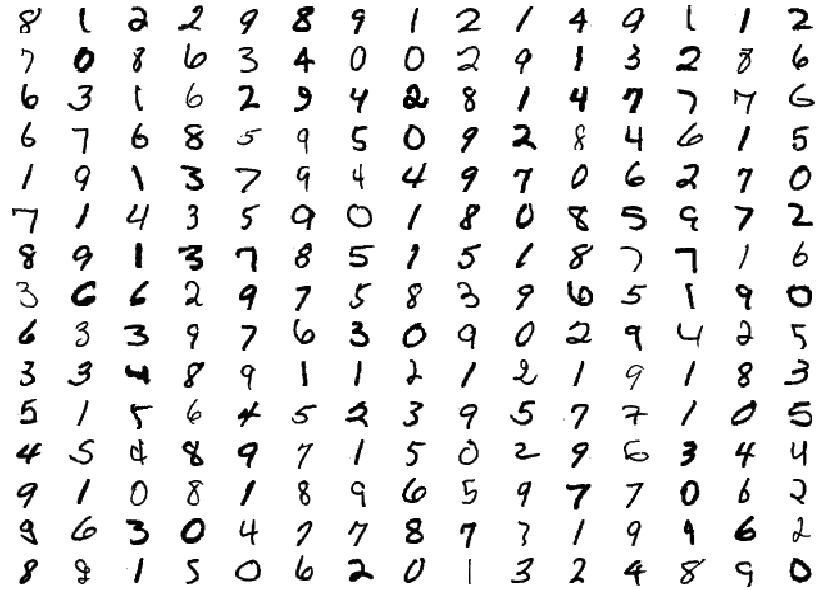
\includegraphics[width=\textwidth]{MNIST_data_examples}
    \caption{Example of 225 randomly chosen digits from the MNIST train set.}
    \label{fig:MNIST_data_examples}
\end{figure}

The MNIST dataset was used in the paper of \citeauthor{Gal2016Active} to compare the performance of approximate Bayesian CNNs with frequentist CNNs in the context of Active Learning. This experiment was replicated in this work by using the same architecture that was explained in \cite{Gal2016Active}.

The experiment consists in starting with a random but balanced sample of 20 images from the MNIST dataset. Next, a CNN is trained with these images, to subsequently take a random sample of 5000 images from the pool set to save computation time. Afterwards, the probability that each of the 5000 images belongs to each of the 10 classes is computed. Finally, the 10 images that maximize the acquisition function are acquired and added to the training set. This process was repeated in 100 acquisition steps for each acquisition function. This whole process is repeated 3 times with different initial images to have the results averaged and reduce the noise inherent in the stochasticity of the process.

The acquisition functions used in the original paper are the Bayesian predictive entropy, frequentist predictive entropy, Bayesian variation ratios, frequentist variation ratios, BALD, random, and an additional one called ``Mean STD'' which was not implemented in this work because of its bad performance in the original paper.

The architecture of the CNN used was convolution-relu-convolution-relu-max pooling-dropout-dense-relu-dropout-dense-softmax, with 32 convolution kernels, $4 \times 4$ kernel size, $2 \times 2$ pooling, dense layer with 128 units, and dropout probabilities $0.25$ and $0.5$. Dropout was only applied to densely connected layers. The CNNs were trained for 50 epochs. For the Bayesian acquisition functions, 100 posterior predictive distribution points were sampled by using the dropout trick mentioned in Chapter \ref{ch:ann}.

The results of the Bayesian and random acquisition functions can be seen in figure \ref{fig:mnist_comparison_active_learning_random}, where the results of our implementation are shown on the left and the original article's results are shown on the right. Our results are very similar with the article's results: apparently, using the variation ratios results in a slightly better performance than BALD or predictive entropy, and more importantly, using the Bayesian acquisition functions results in a much better performance than using a random acquisition function.

\begin{figure}[H]
    \centering
    \subfloat[Our results.]{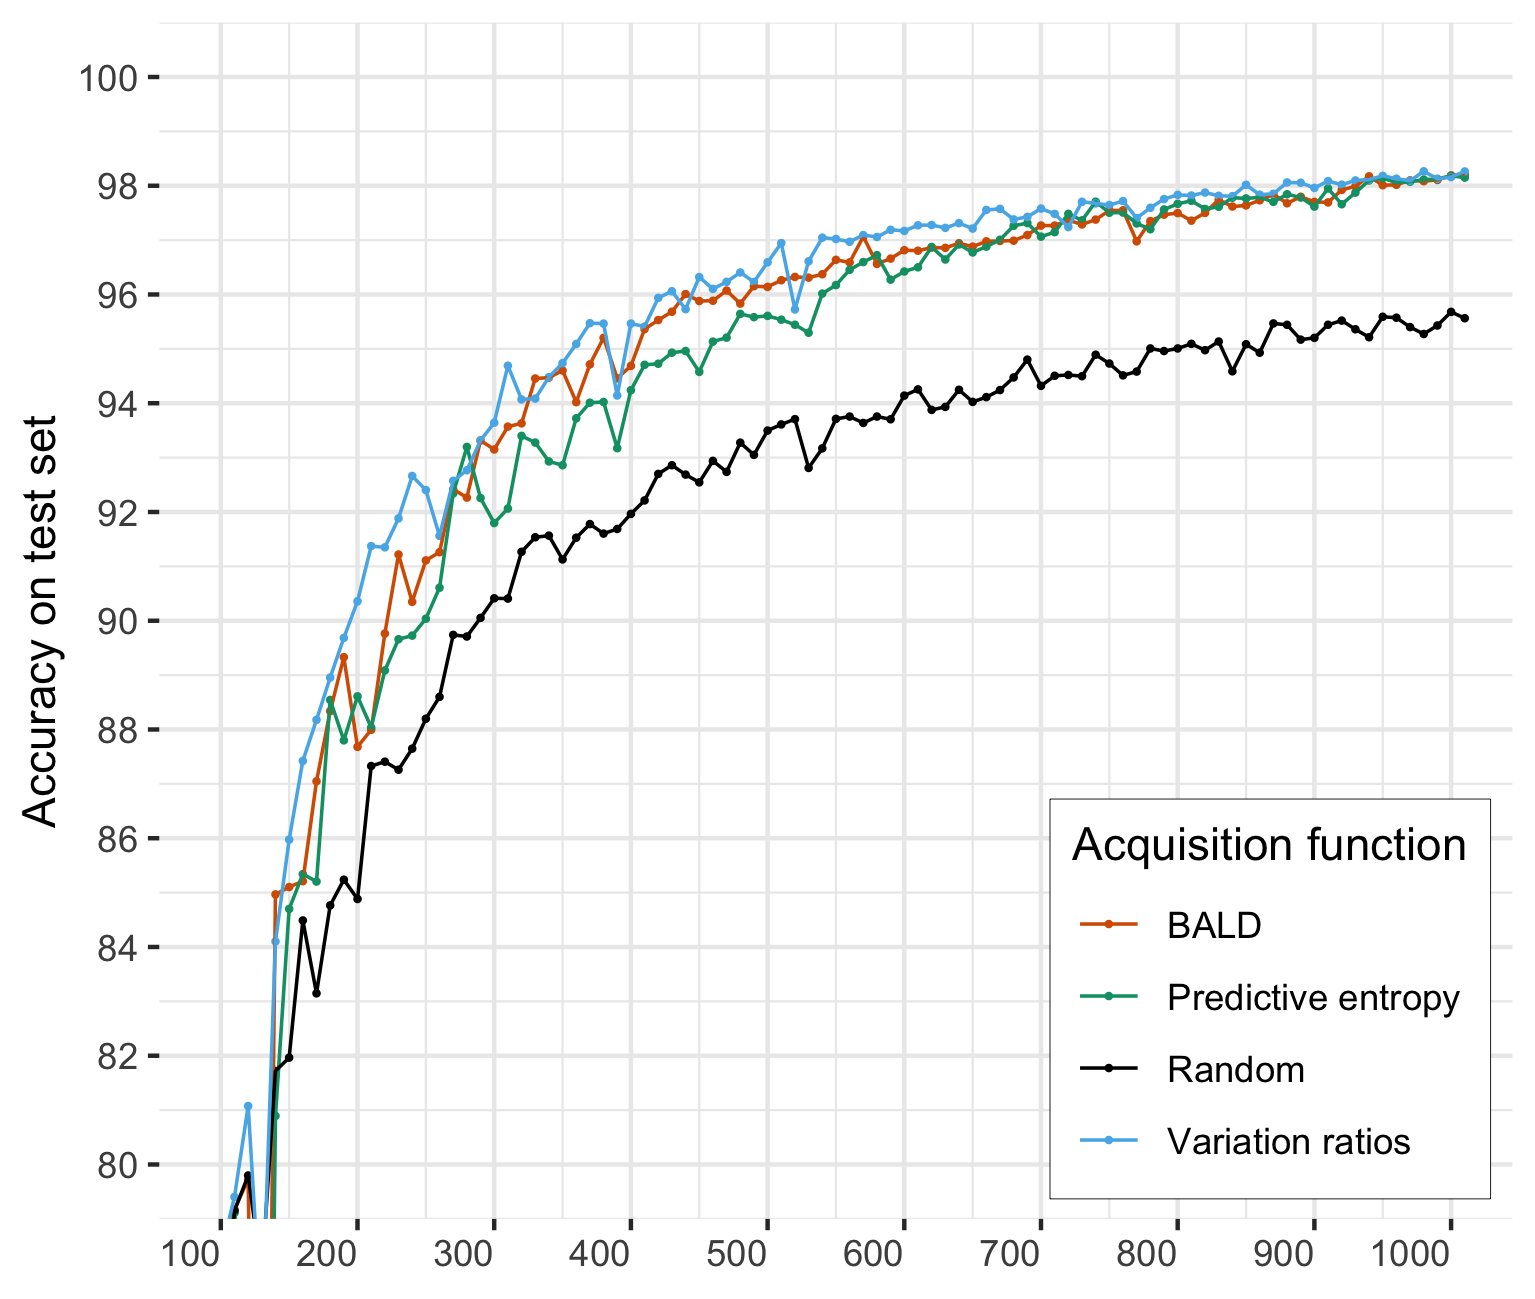
\includegraphics[width=0.5\textwidth]{MNIST_accuracies_bayesian}}
    \hfill
    \subfloat[Paper's results.]{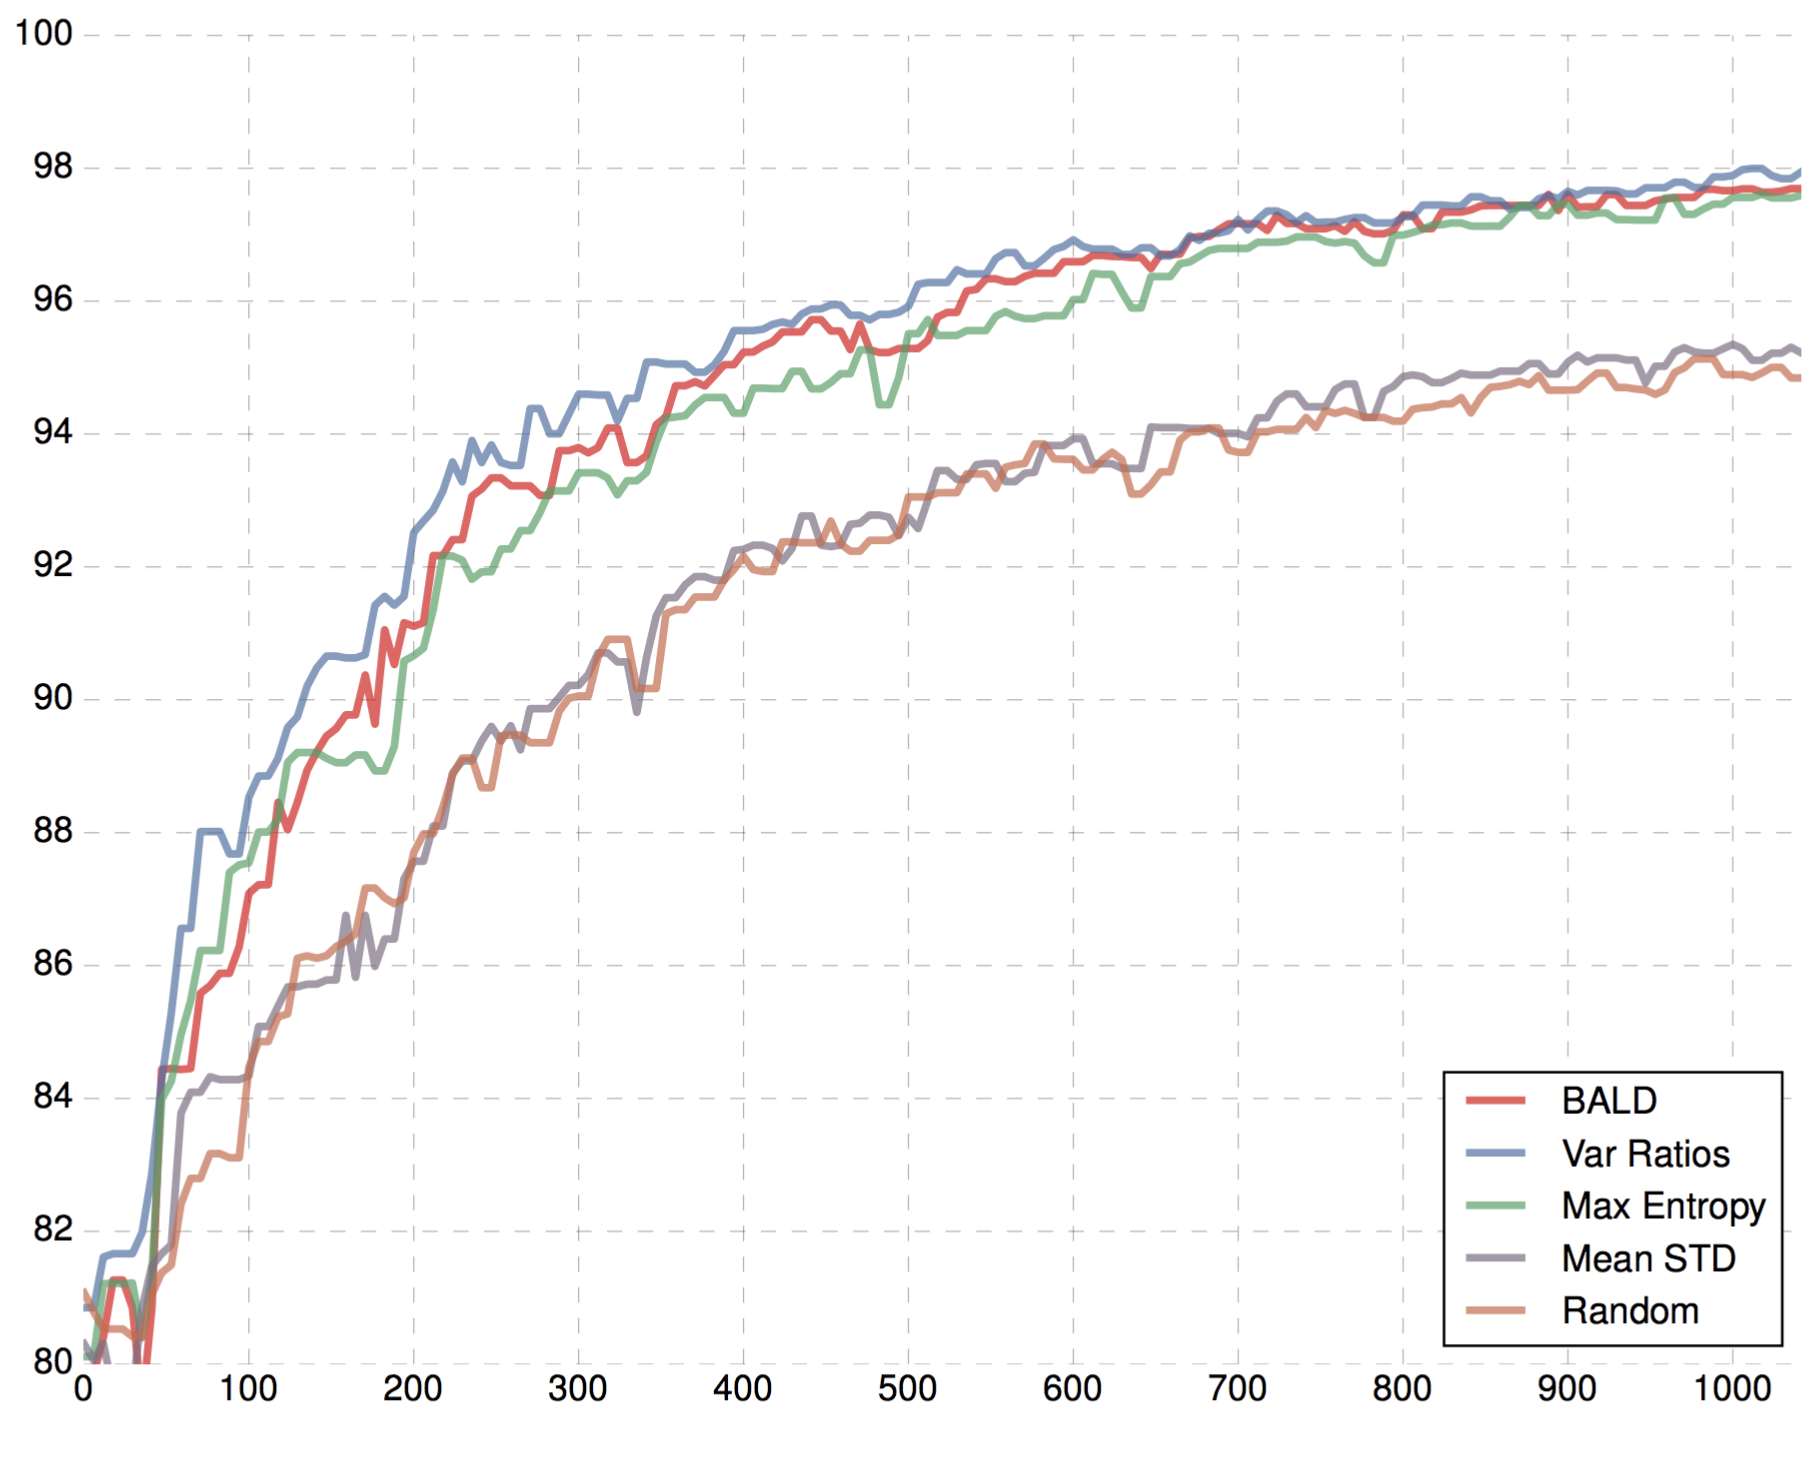
\includegraphics[width=0.5\textwidth]{MNIST_all_gal_islam}}
    \caption{Accuracy of models in each acquisition step. The left picture shows our implementation and the right picture shows \citeauthor{Gal2016Active}'s implementation. The $x$ axis is the number of images.}
    \label{fig:mnist_comparison_active_learning_random}
\end{figure}

Our implementation achieved the goal of outperforming a random acquisition function. However, the results differ when one compares the Bayesian and the frequentist approach. The article's authors claim that the use of an approximate Bayesian approach in the acquisition process of Active Learning leads to better accuracy with fewer images, but in our implementation this does not happen. This can be seen with more detail in figures in \ref{fig:mnist_pred_entropy_AL} and \ref{fig:mnist_var_ratios_AL} that show our results on the left and the paper's results on the right. In the original paper, the frequentist acquisition functions lead to a worse performance than their Bayesian counterparts, while in our implementation there is no evidence of distinction between the two.

For example, with predictive entropy in figure \ref{fig:mnist_pred_entropy_AL}, the results seem to be backward and the frequentist acquisition function seems to have a slightly better performance that the Bayesian one. Another difference is that the frequentist acquisition function in the original article achieves a 90\% accuracy with around 300 images, while in our implementation this accuracy is first achieved with around 200 images.

\begin{figure}[H]
  \centering
  \subfloat[Our results.]{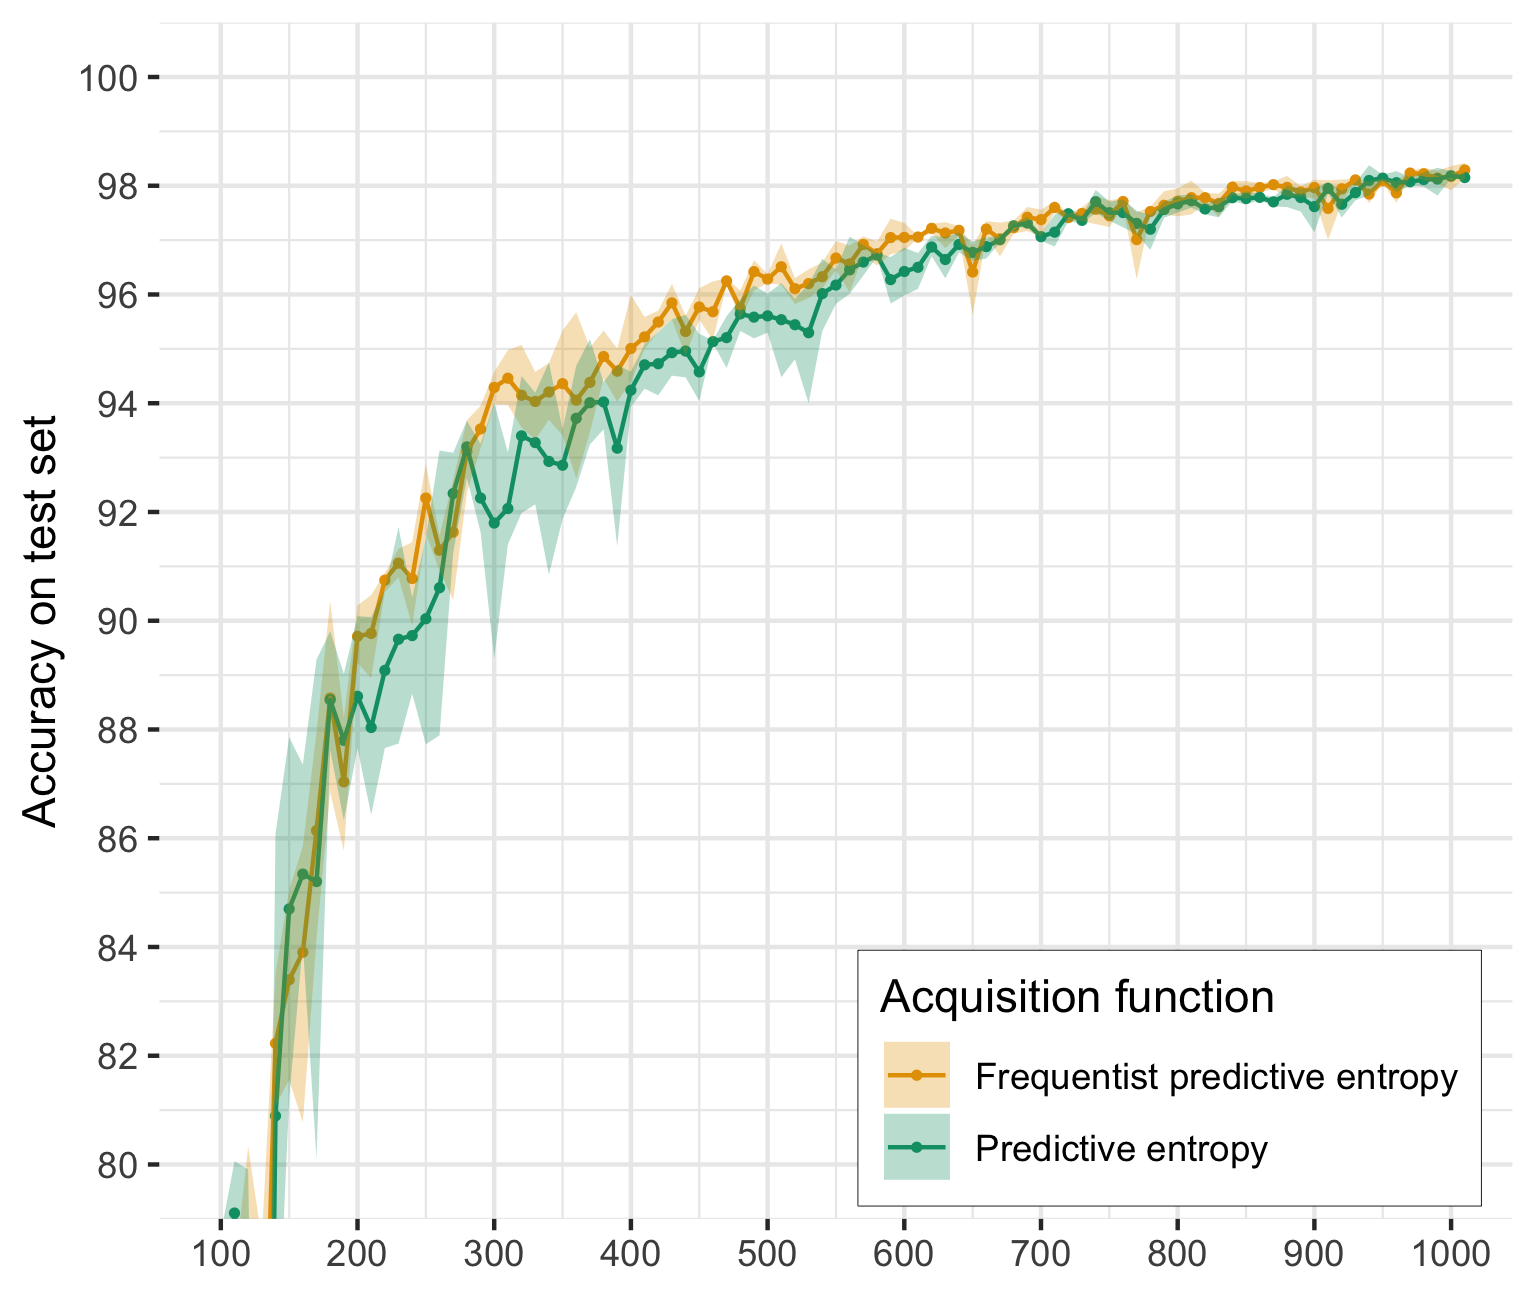
\includegraphics[width=0.5\textwidth]{MNIST_accuracies_pred_ent_ribbon}}
  \hfill
  \subfloat[Paper's results.]{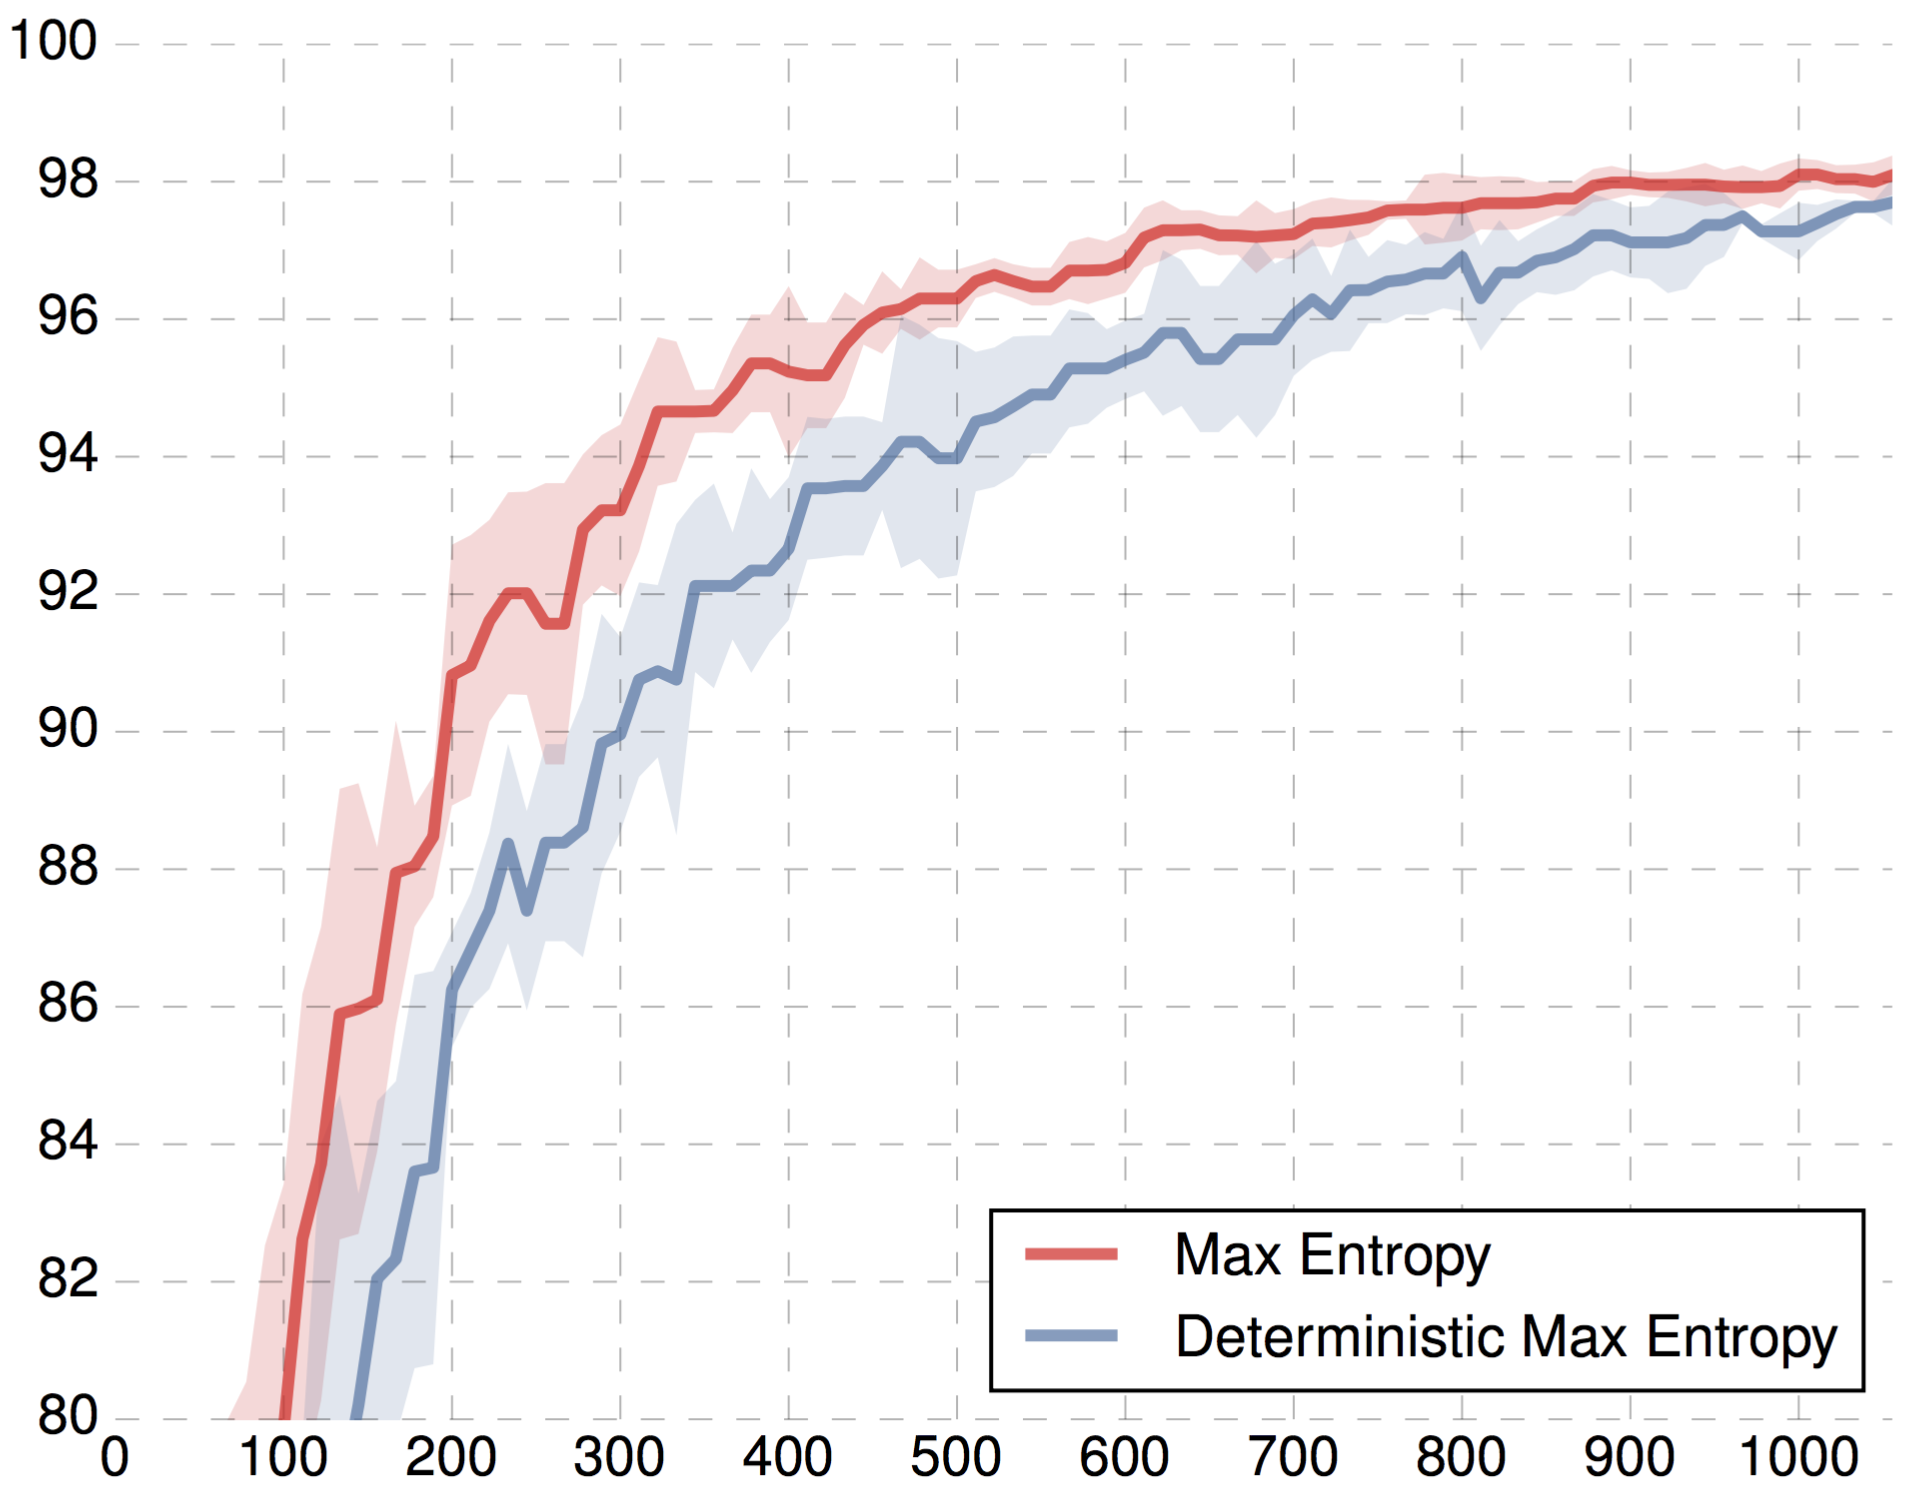
\includegraphics[width=0.5\textwidth]{MNIST_pred_ent_gal_islam}}
  \caption{Accuracy of approximate Bayesian and frequentist models in each acquisition step using predictive entropy as acquisition function. The left picture shows our implementation and the right picture shows \citeauthor{Gal2016Active}'s implementation.}
  \label{fig:mnist_pred_entropy_AL}
\end{figure}

Figure \ref{fig:mnist_var_ratios_AL} shows the results of the variation ratios acquisition functions. While the roles of the frequentist and Bayesian acquisition functions are not reversed as in the previous case, there is apparently no distinction between the two acquisition functions. Moreover, in the original article, a 90\% accuracy is first achieved using the frequentist acquisition function with a little below 300 images, while in our implementation this accuracy is first achieved with around 200 images. Another difference is that with 1000 images and using the frequentist acquisition function, the authors' accuracy is close to 96\%, while in our implementation it is close to 98\%.

\begin{figure}[H]
  \centering
  \subfloat[Our results.]{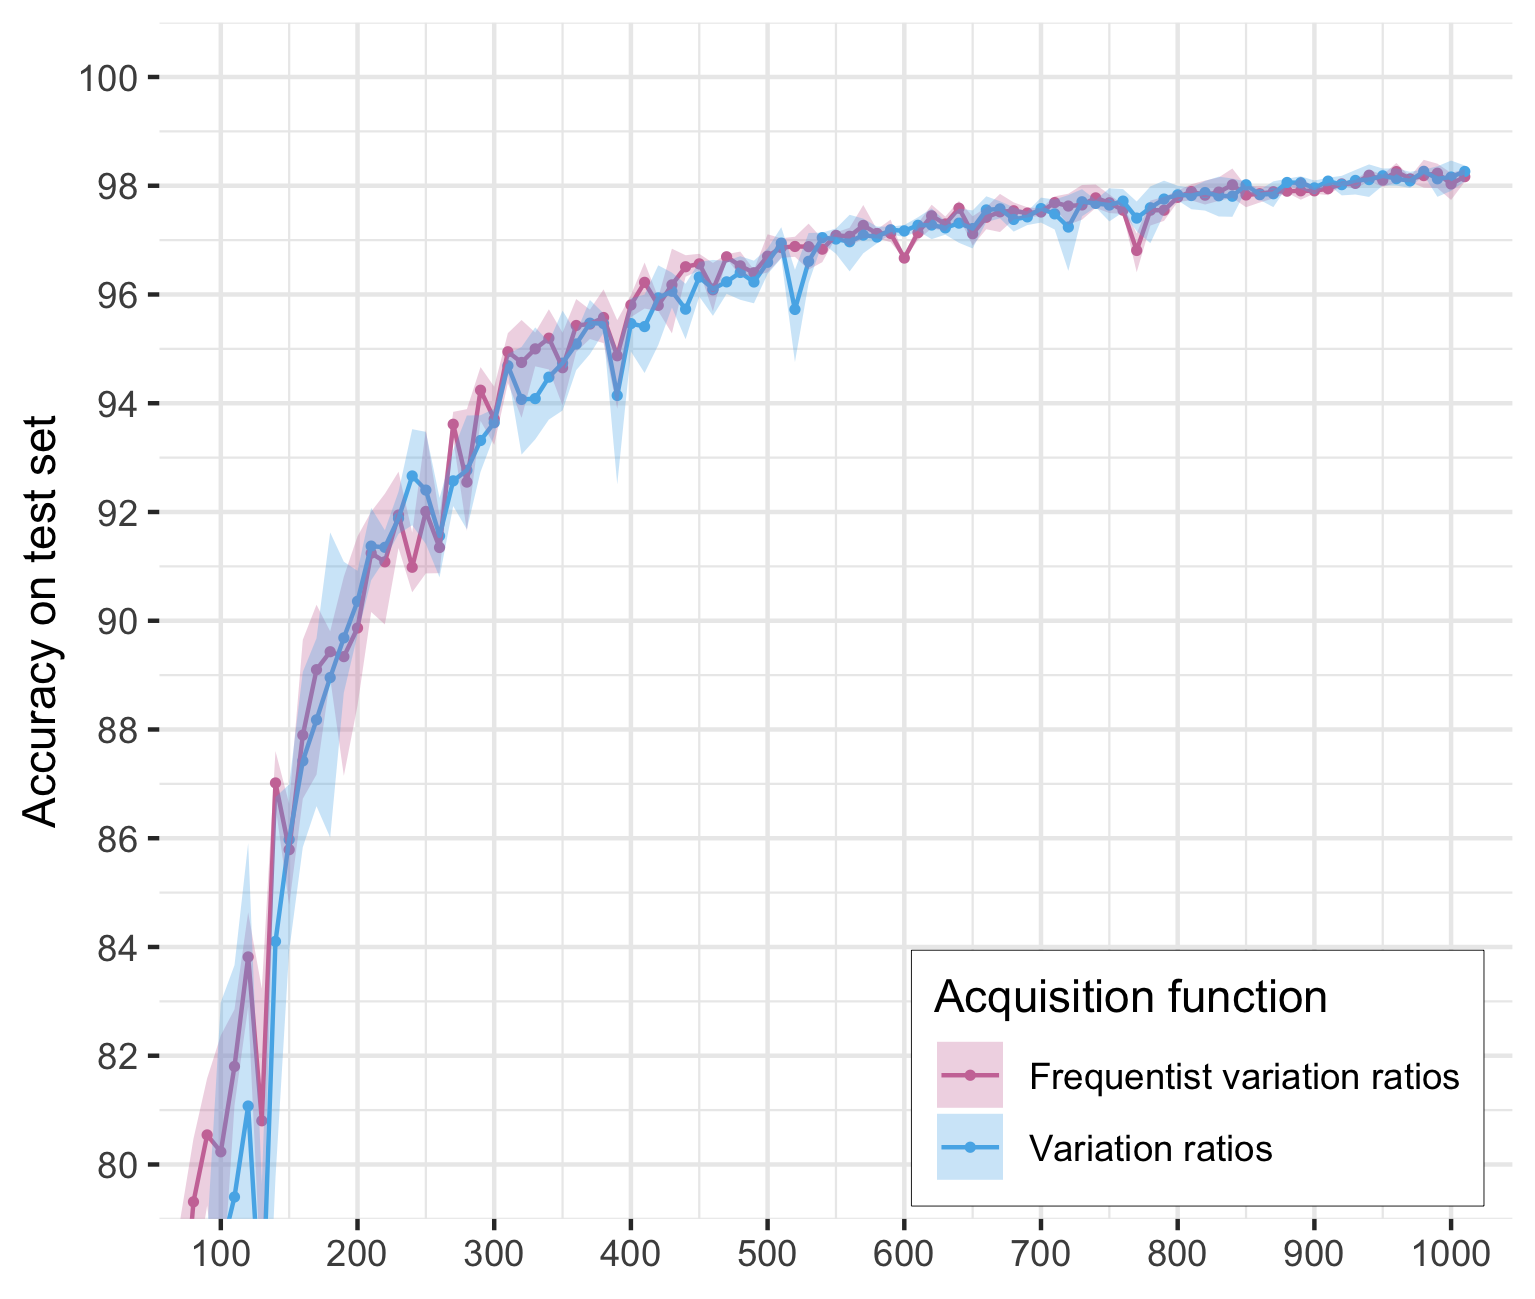
\includegraphics[width=0.5\textwidth]{MNIST_accuracies_var_ratios_ribbon}}
  \hfill
  \subfloat[Paper's results.]{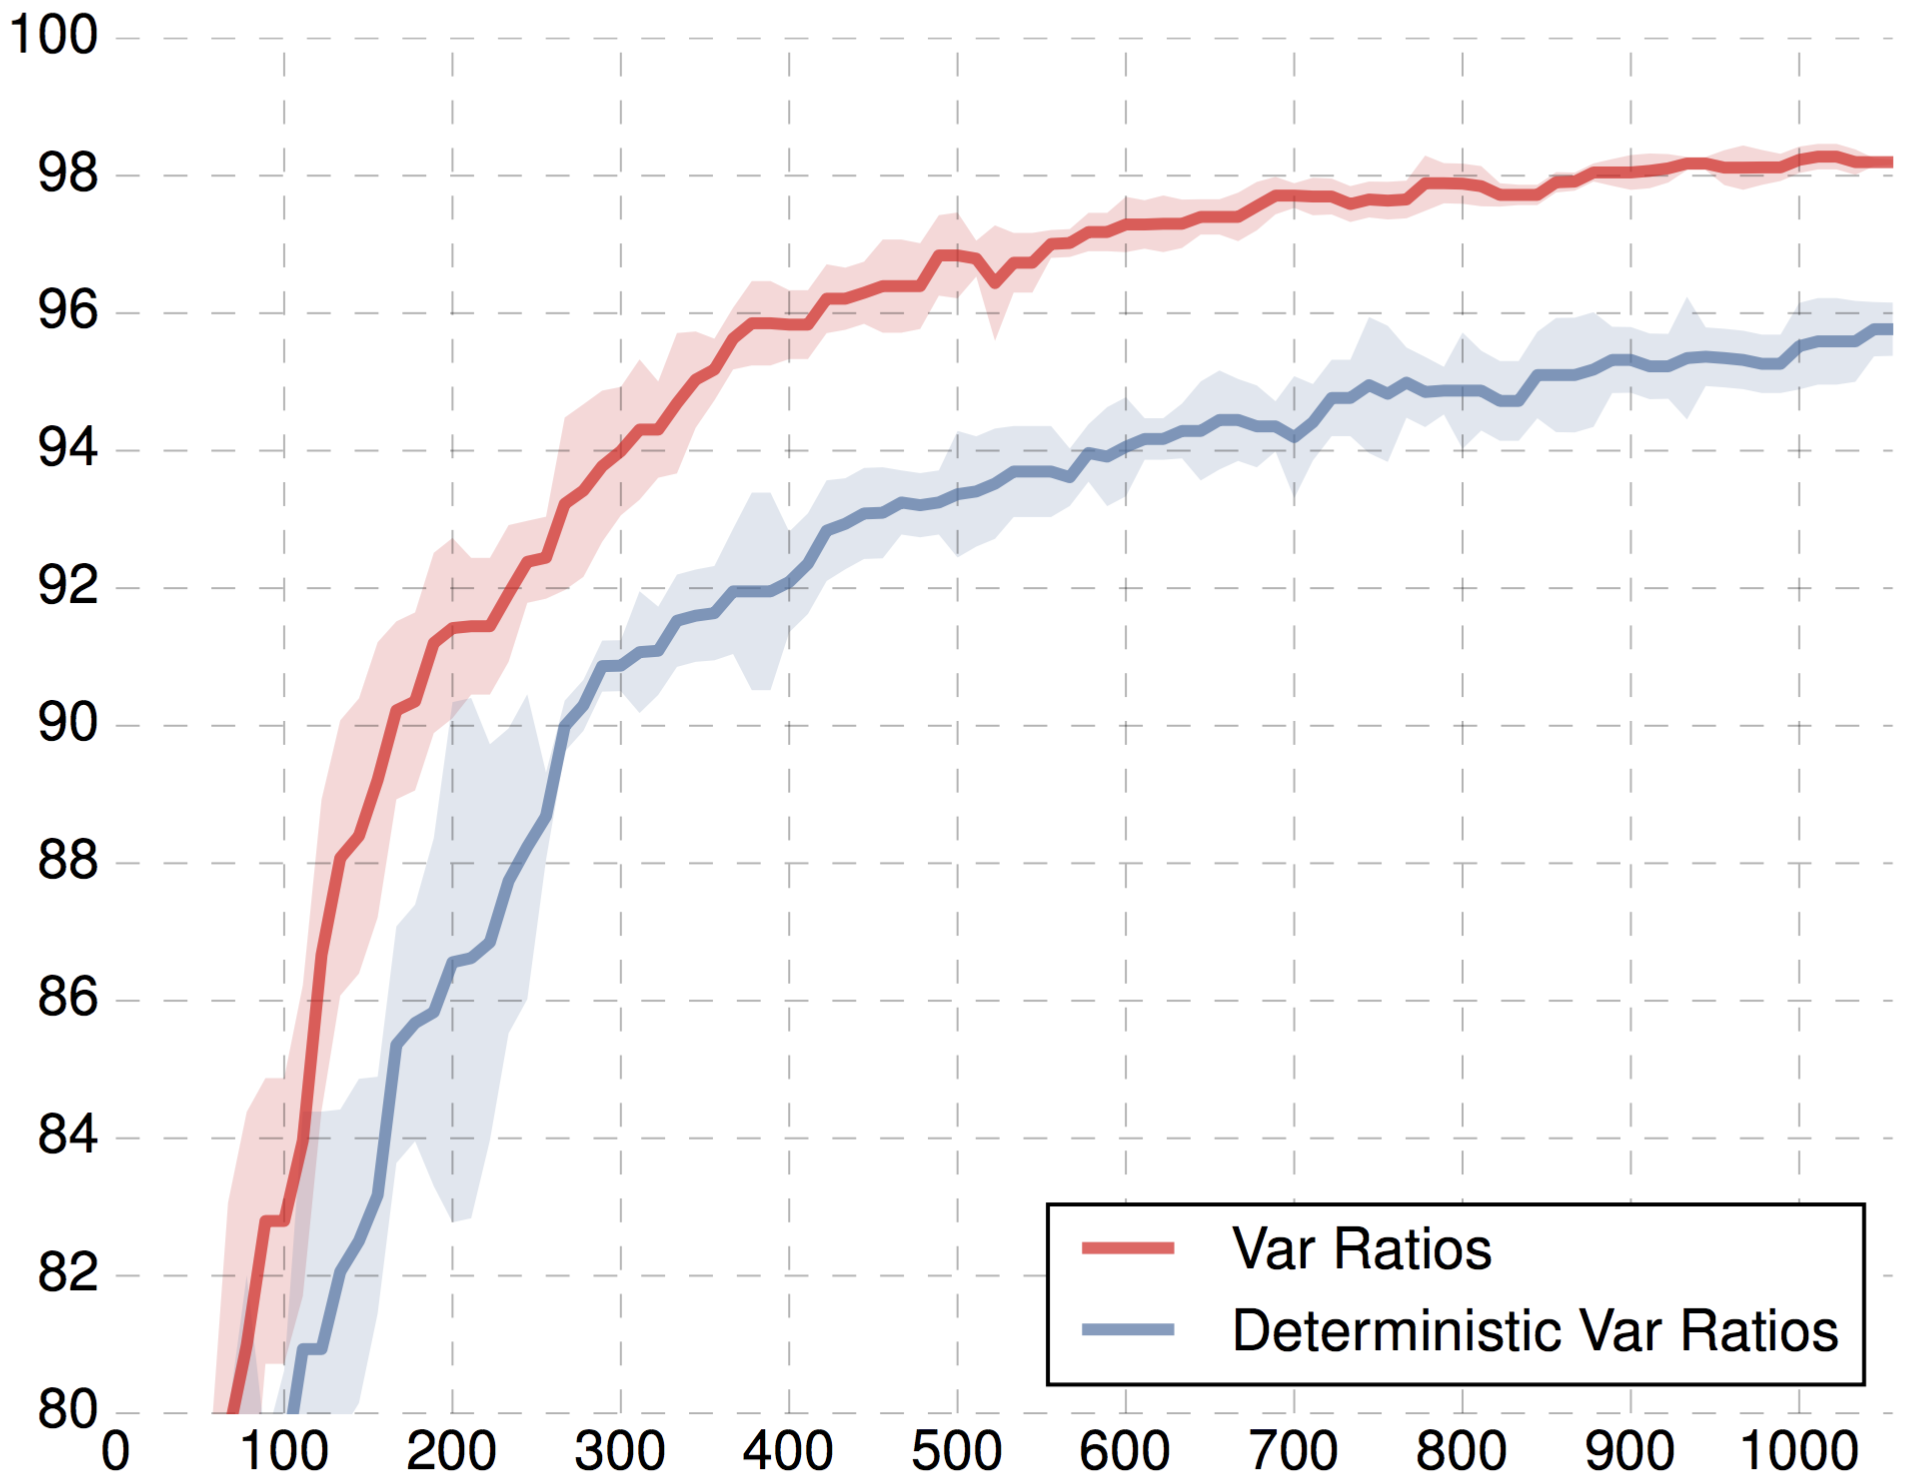
\includegraphics[width=0.5\textwidth]{MNIST_var_ratios_gal_islam}}
  \caption{Accuracy of approximate Bayesian and frequentist models in each acquisition step using variation ratios as acquisition function. The left picture shows our implementation and the right picture shows \citeauthor{Gal2016Active}'s implementation.}
  \label{fig:mnist_var_ratios_AL}
\end{figure}


%%%%%%%%%%%%%%%%%%%%%%%%%%%%%%%%%%%%%%%%%%%%%%%%%%%%%%%%%%%%%%
%%%%%%%%%%%%%%%%%%%%%%%%%%%%%%%%%%%%%%%%%%%%%%%%%%%%%%%%%%%%%%
\section{Cats and dogs dataset}
%%%%%%%%%%%%%%%%%%%%%%%%%%%%%%%%%%%%%%%%%%%%%%%%%%%%%%%%%%%%%%
%%%%%%%%%%%%%%%%%%%%%%%%%%%%%%%%%%%%%%%%%%%%%%%%%%%%%%%%%%%%%%

The cats and dogs dataset was first used for a CAPTCHA developed by Microsoft Research called Asirra \cite{elson2007asirra}. It is a collection of \numprint{25000} pictures of size $64 \times 64$, of which half are cats and half are dogs. Figure \ref{fig:cats_dogs_data_examples} shows 30 randomly chosen cats and 30 randomly chosen dogs from the training set.

\begin{figure}[H]
    \centering
    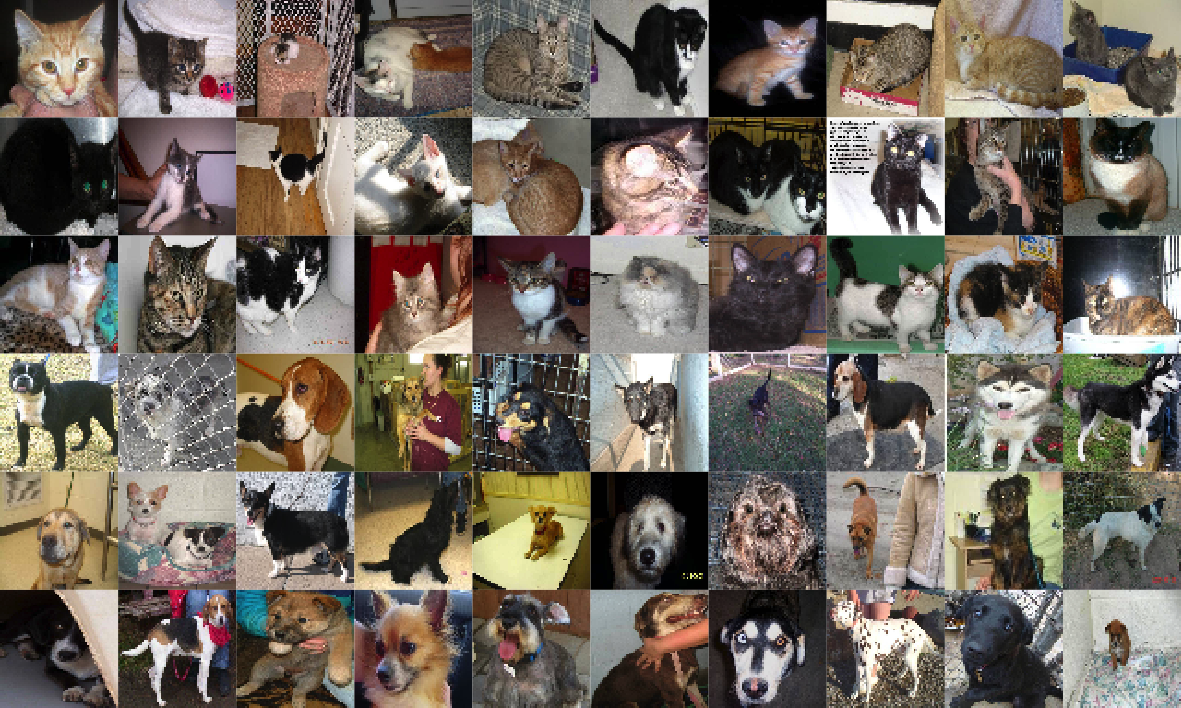
\includegraphics[width=\textwidth]{cats_dogs_data_examples}
    \caption{Example of 60 randomly chosen cats and 30 randomly chosen dogs from the dataset.}
    \label{fig:cats_dogs_data_examples}
\end{figure}

The process of this experiment is very similar to the one followed in the MNIST dataset. First, a balanced set of 100 images was randomly chosen and used to train a first model. Then a random sample of 2000 images was chosen from the pool set, from which the predicted probabilities of belonging to each class were computed. Subsequently, the 50 images with the highest acquisition function value were chosen and added to the training set. The final number of acquisition steps was 50 and, once more, the whole process was repeated 3 times with different initial images.

The architecture used was convolution-relu-convolution-relu-max pooling-dropout-convolution-relu-max pooling-dropout-dense-relu-dropout-dense-softmax with 32 convolution kernels, $3 \times 3$ kernel size, $2 \times 2$ pooling, dense layer with 64 units, and dropout probabilities $0.25$, $0.25$ and $0.5$. The CNNs were trained for 200 epochs. Once more, for the Bayesian acquisition functions 100 posterior predictive distribution points were sampled by using the dropout trick.

The results of the Bayesian and random acquisition functions can be seen in figure \ref{fig:cats_dogs_accuracies_bayesian}. In this case, it is difficult to say that using any of the Bayesian acquisition functions results in a better performance than using a random acquisition function. In the last steps it is clear that the variation ratios acquisition function results in a better accuracy, but the difference is not as abrupt as it was in the MNIST dataset.

\begin{figure}[H]
    \centering
    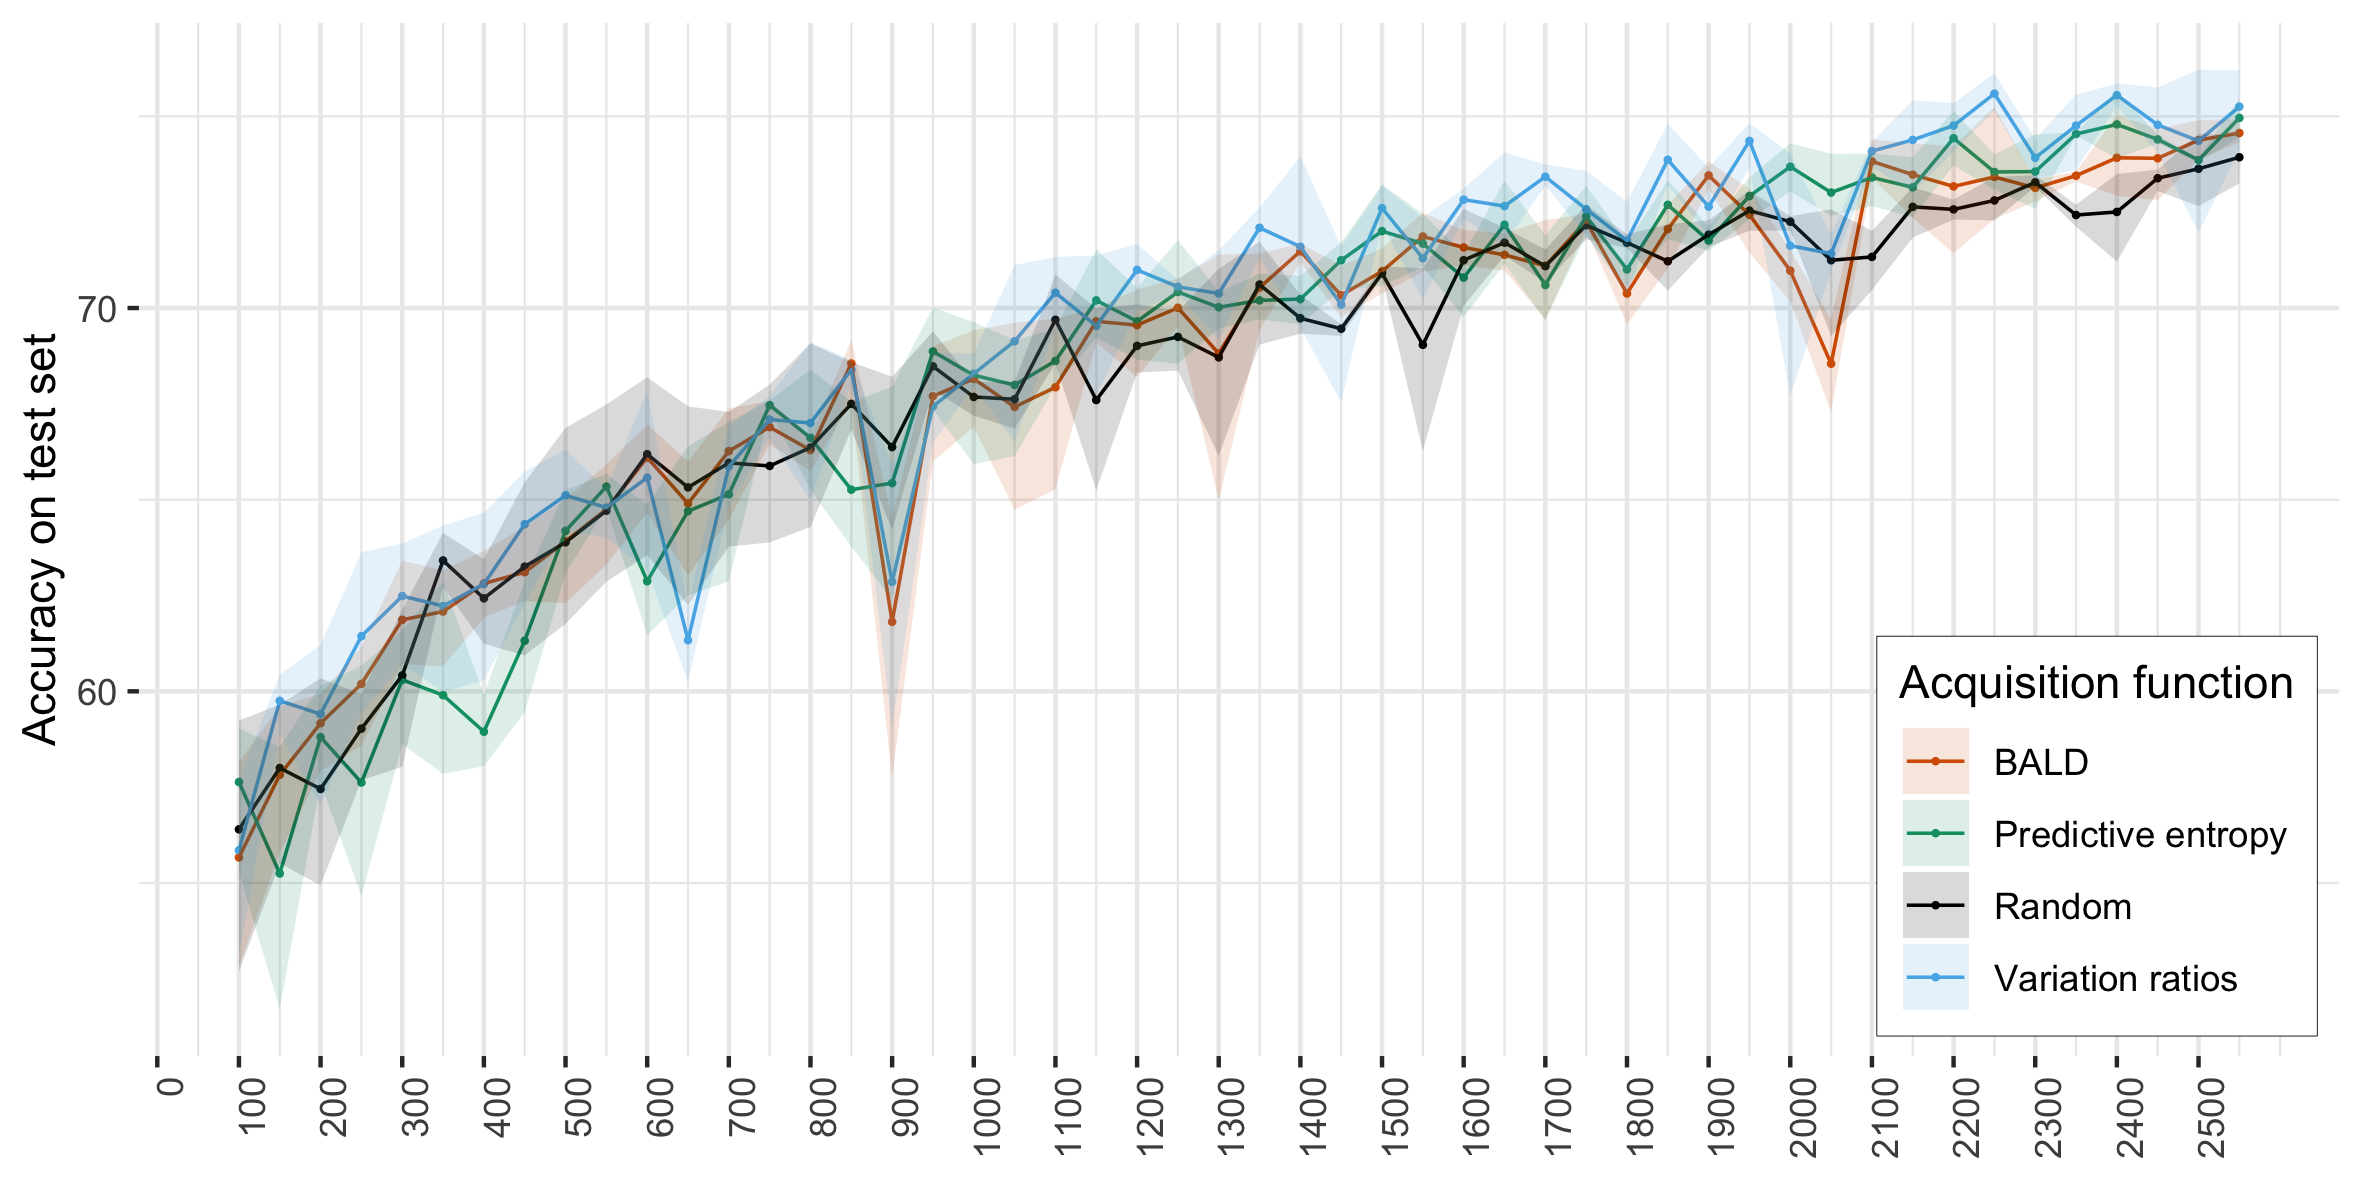
\includegraphics[width=\textwidth]{cats_dogs_accuracies_bayesian_shaded}
    \caption{Accuracy of models in each acquisition step in the cats and dogs dataset.}
    \label{fig:cats_dogs_accuracies_bayesian}
\end{figure}

Figure \ref{fig:cats_dogs_bayesian_vs_freq} shows the comparison of the frequentist and Bayesian acquisition functions, with predictive entropy on the left and variation ratios on the right. As with the MNIST dataset, there is no clear distinction between the frequentist and the Bayesian acquisition functions.

\begin{figure}[H]
    \centering
    \subfloat[Predictive entropy.]{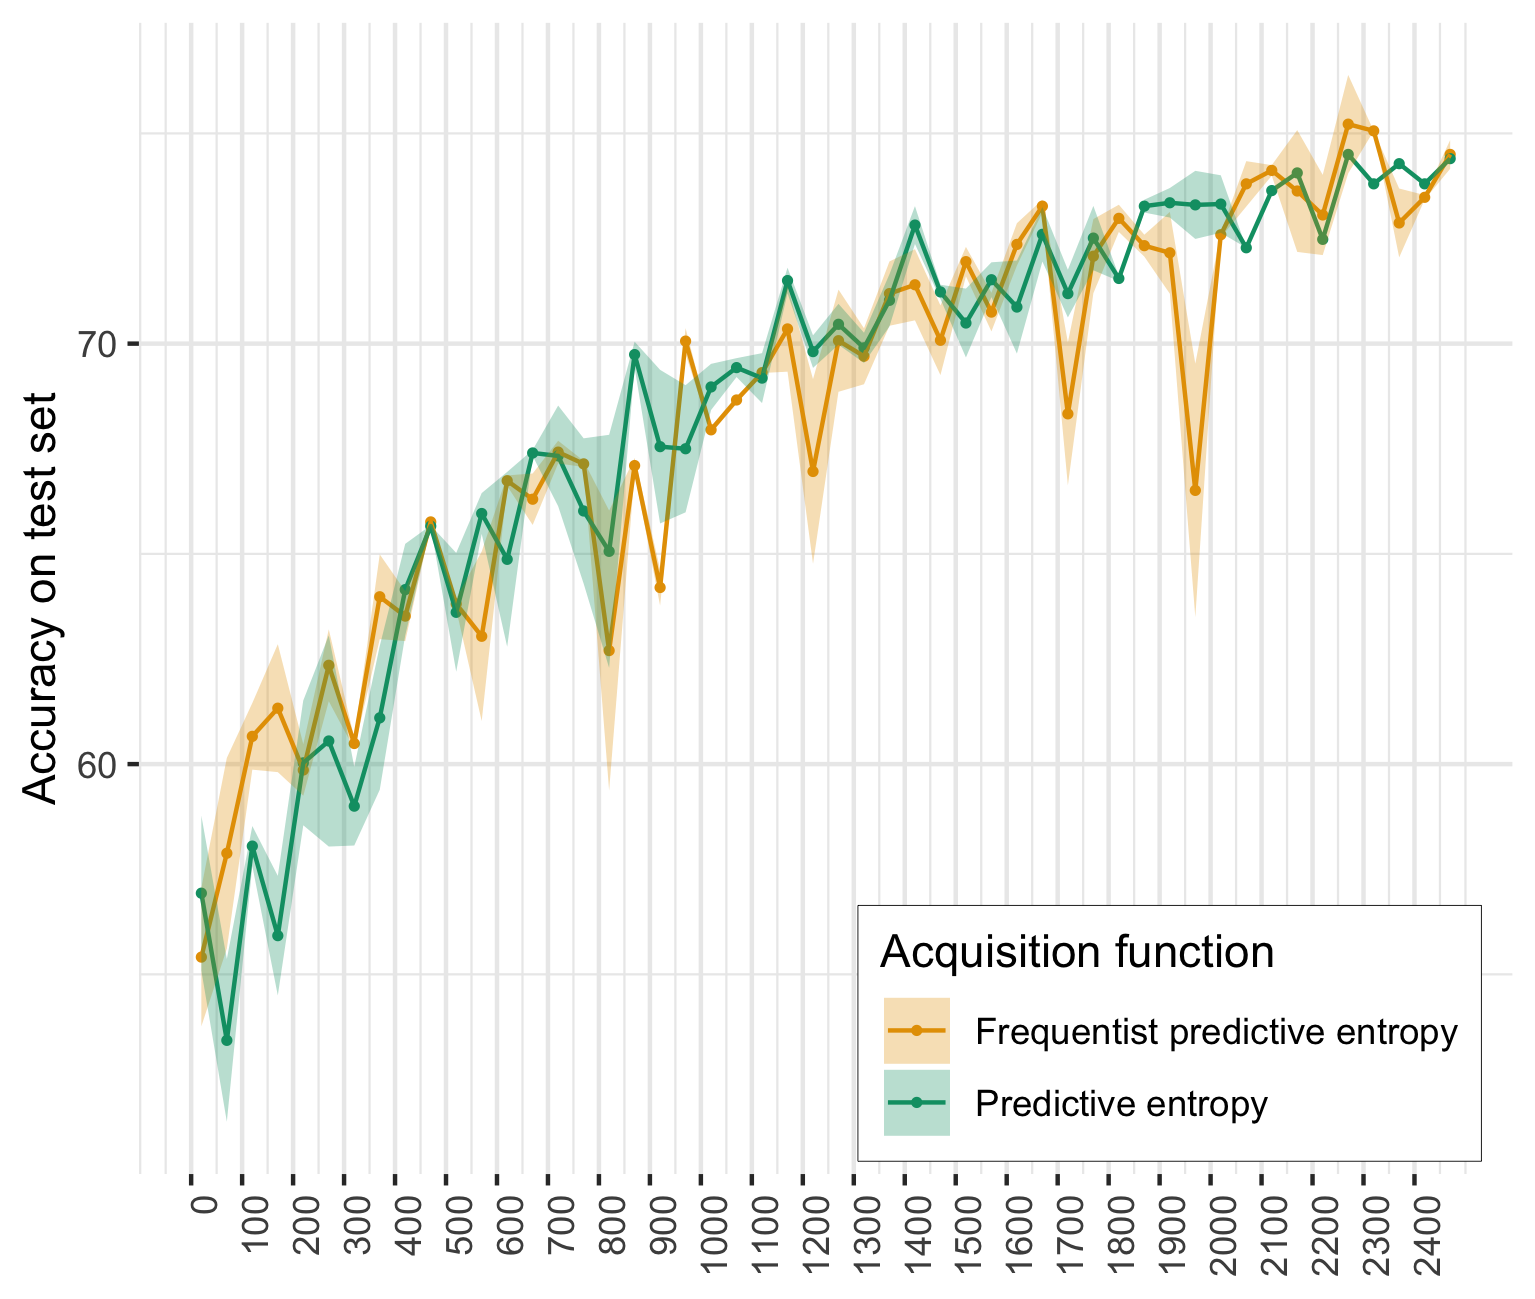
\includegraphics[width=0.5\textwidth]{cats_dogs_accuracies_pred_ent_ribbon}}
    \hfill
    \subfloat[Variation ratios.]{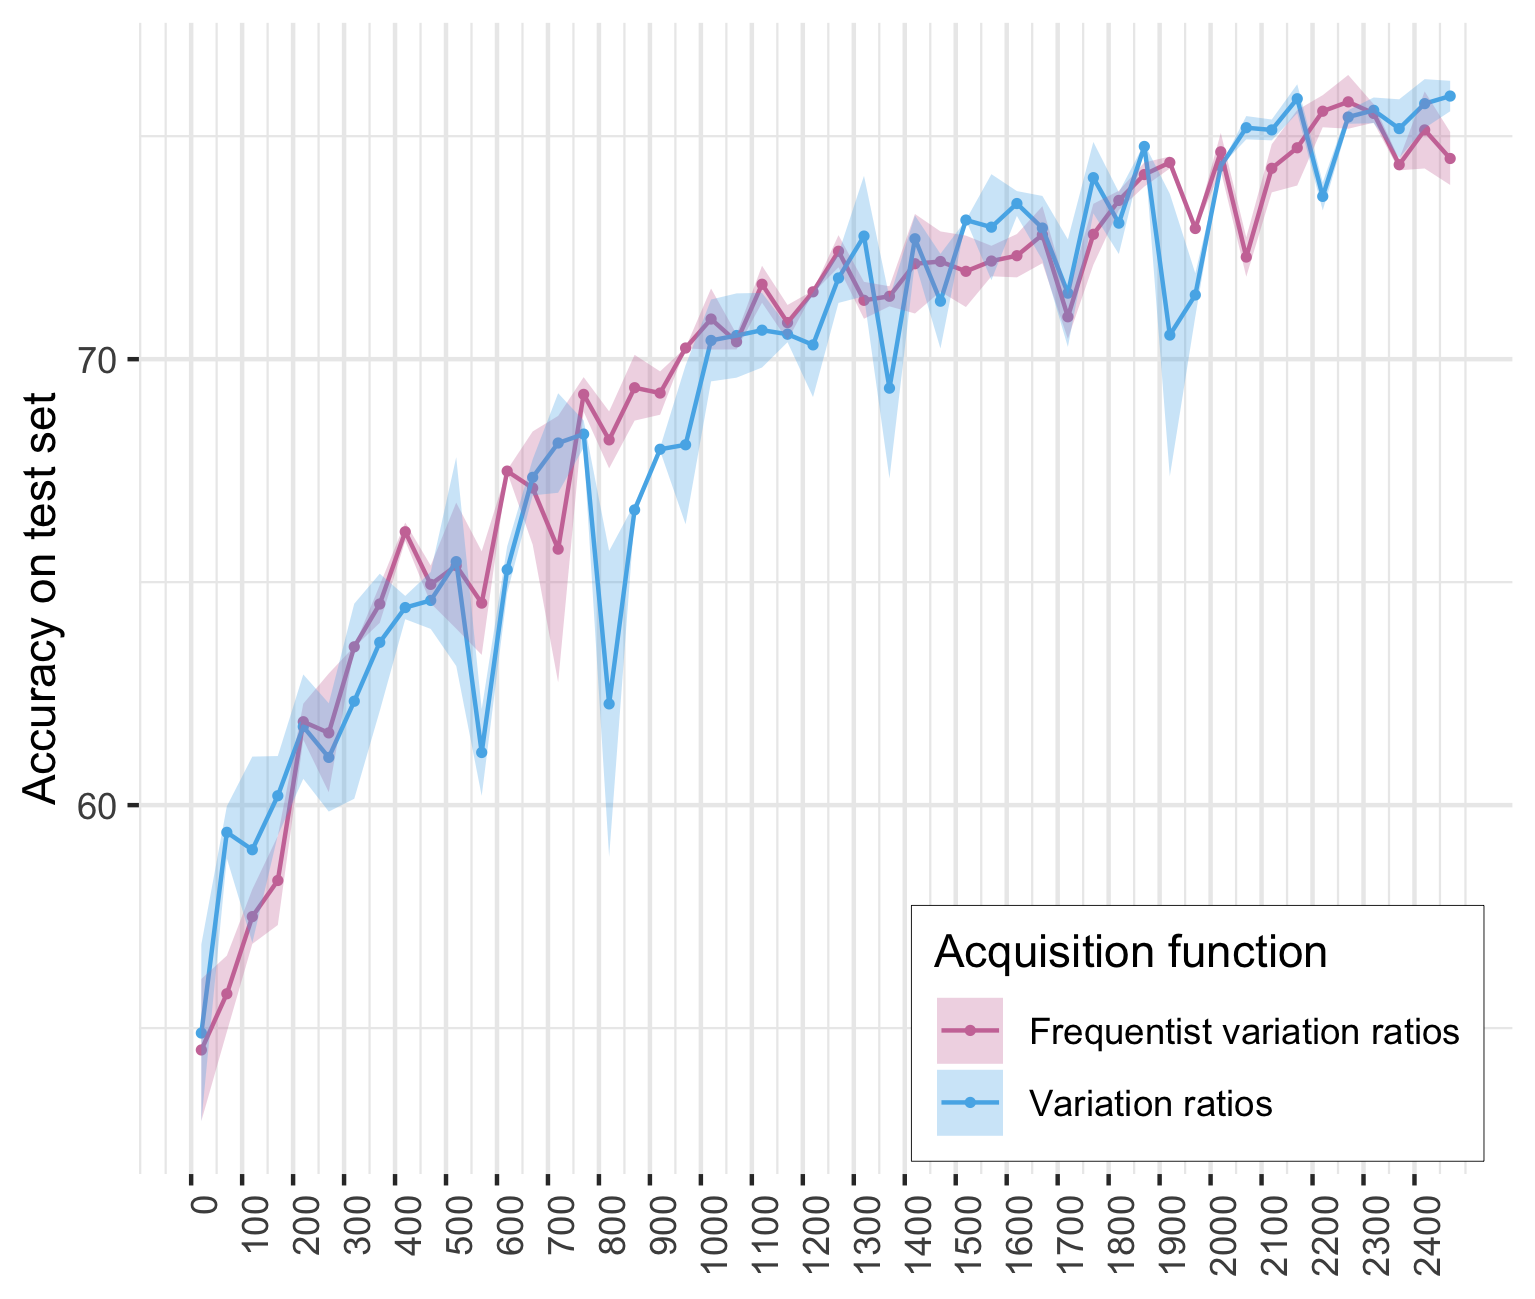
\includegraphics[width=0.5\textwidth]{cats_dogs_accuracies_var_ratios_ribbon}}
    \caption{Accuracy of models in each acquisition step in the cats and dogs dataset.}
    \label{fig:cats_dogs_bayesian_vs_freq}
\end{figure}




%%%%%%%%%%%%%%%%%%%%%%%%%%%%%%%%%%%%%%%%%%%%%%%%%%%%%%%%%%%%%%
%%%%%%%%%%%%%%%%%%%%%%%%%%%%%%%%%%%%%%%%%%%%%%%%%%%%%%%%%%%%%%
\section{CIFAR-10 dataset}
%%%%%%%%%%%%%%%%%%%%%%%%%%%%%%%%%%%%%%%%%%%%%%%%%%%%%%%%%%%%%%
%%%%%%%%%%%%%%%%%%%%%%%%%%%%%%%%%%%%%%%%%%%%%%%%%%%%%%%%%%%%%%

The CIFAR10 was introduced in \citeyear{krizhevsky2009learning}. The name stands for the Canadian Institute for Advanced Research, who funded the project in which it was first used \cite{krizhevsky2009learning}. It consists of \numprint{60000} color images of size $32 \times 32$ representing 10 different types of objects, these being \textit{airplane}, \textit{automobile}, \textit{bird}, \textit{cat}, \textit{deer}, \textit{dog}, \textit{frog}, \textit{horse}, \textit{ship} and \textit{truck}. The classes are balanced in the dataset, meaning that each class has the same number of images. Of the \numprint{60000} images, \numprint{50000} are used as a training set and the rest as test set. The training set and the test are also balanced. Figure \ref{fig:CIFAR10_data_examples} shows 200 randomly chosen images from the training set.

\begin{figure}[H]
    \centering
    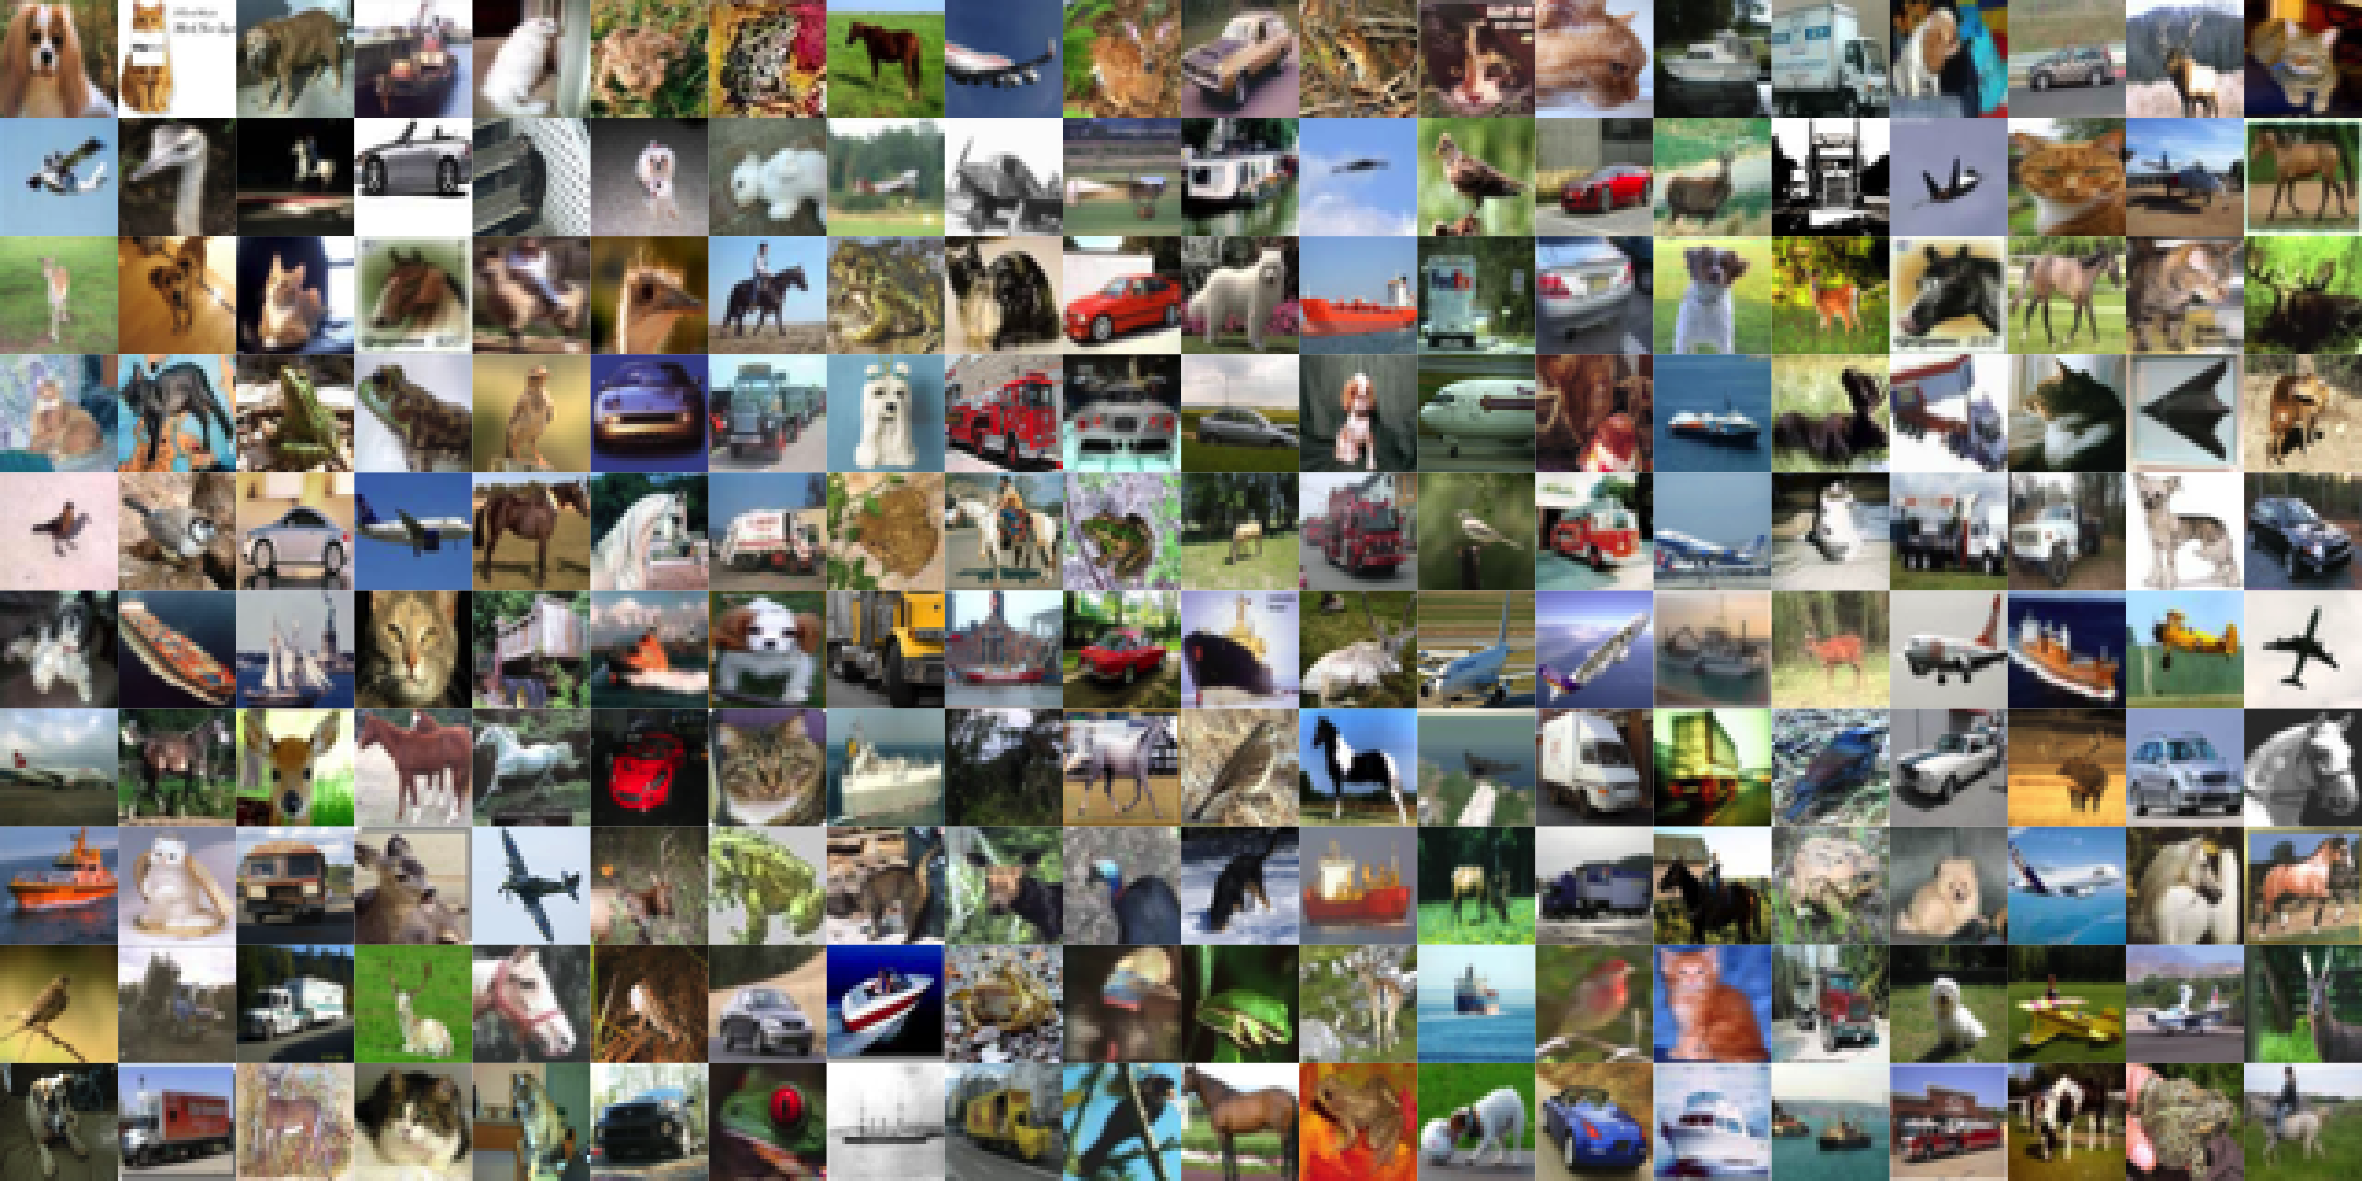
\includegraphics[width=\textwidth]{CIFAR10_data_examples}
    \caption{Example of 200 randomly chosen images from the dataset.}
    \label{fig:CIFAR10_data_examples}
\end{figure}

The process of this last experiment is very similar to the ones followed in the two previous datasets. First, as in the cats and dogs dataset, a balanced set of 100 images was randomly chosen and used to train a first model. Then a random sample of 5000 images was chosen from the pool set, from which the predicted probabilities of belonging to each class were computed. Afterwards, the 1000 images with the highest acquisition function value were chosen and added to the training set. The final number of acquisition steps was 40 and, as before, the whole process was repeated 3 times with different initial images.

The architecture used was convolution-relu-convolution-relu-max pooling-dropout-convolution-relu-convolution-relu-max pooling-dropout-dense-relu-dropout-dense-softmax with 32 convolution kernels, $3 \times 3$ kernel size, $2 \times 2$ pooling, dense layer with 512 units, and dropout probabilities $0.25$, $0.25$ and $0.5$. The CNNs were trained for 100 epochs. Like in the previous experiments, for the Bayesian acquisition functions 100 posterior predictive distribution points were sampled by using the dropout trick.

The results of the Bayesian and random acquisition functions can be seen in figure \ref{fig:CIFAR10_accuracies_bayesian}. Here, the difference between the random acquisition function and the rest is a little clearer than in the cats and dogs dataset, especially from around the \numprint{13000} image mark onward, but it is not as clear as in the MNIST dataset.

\begin{figure}[H]
    \centering
    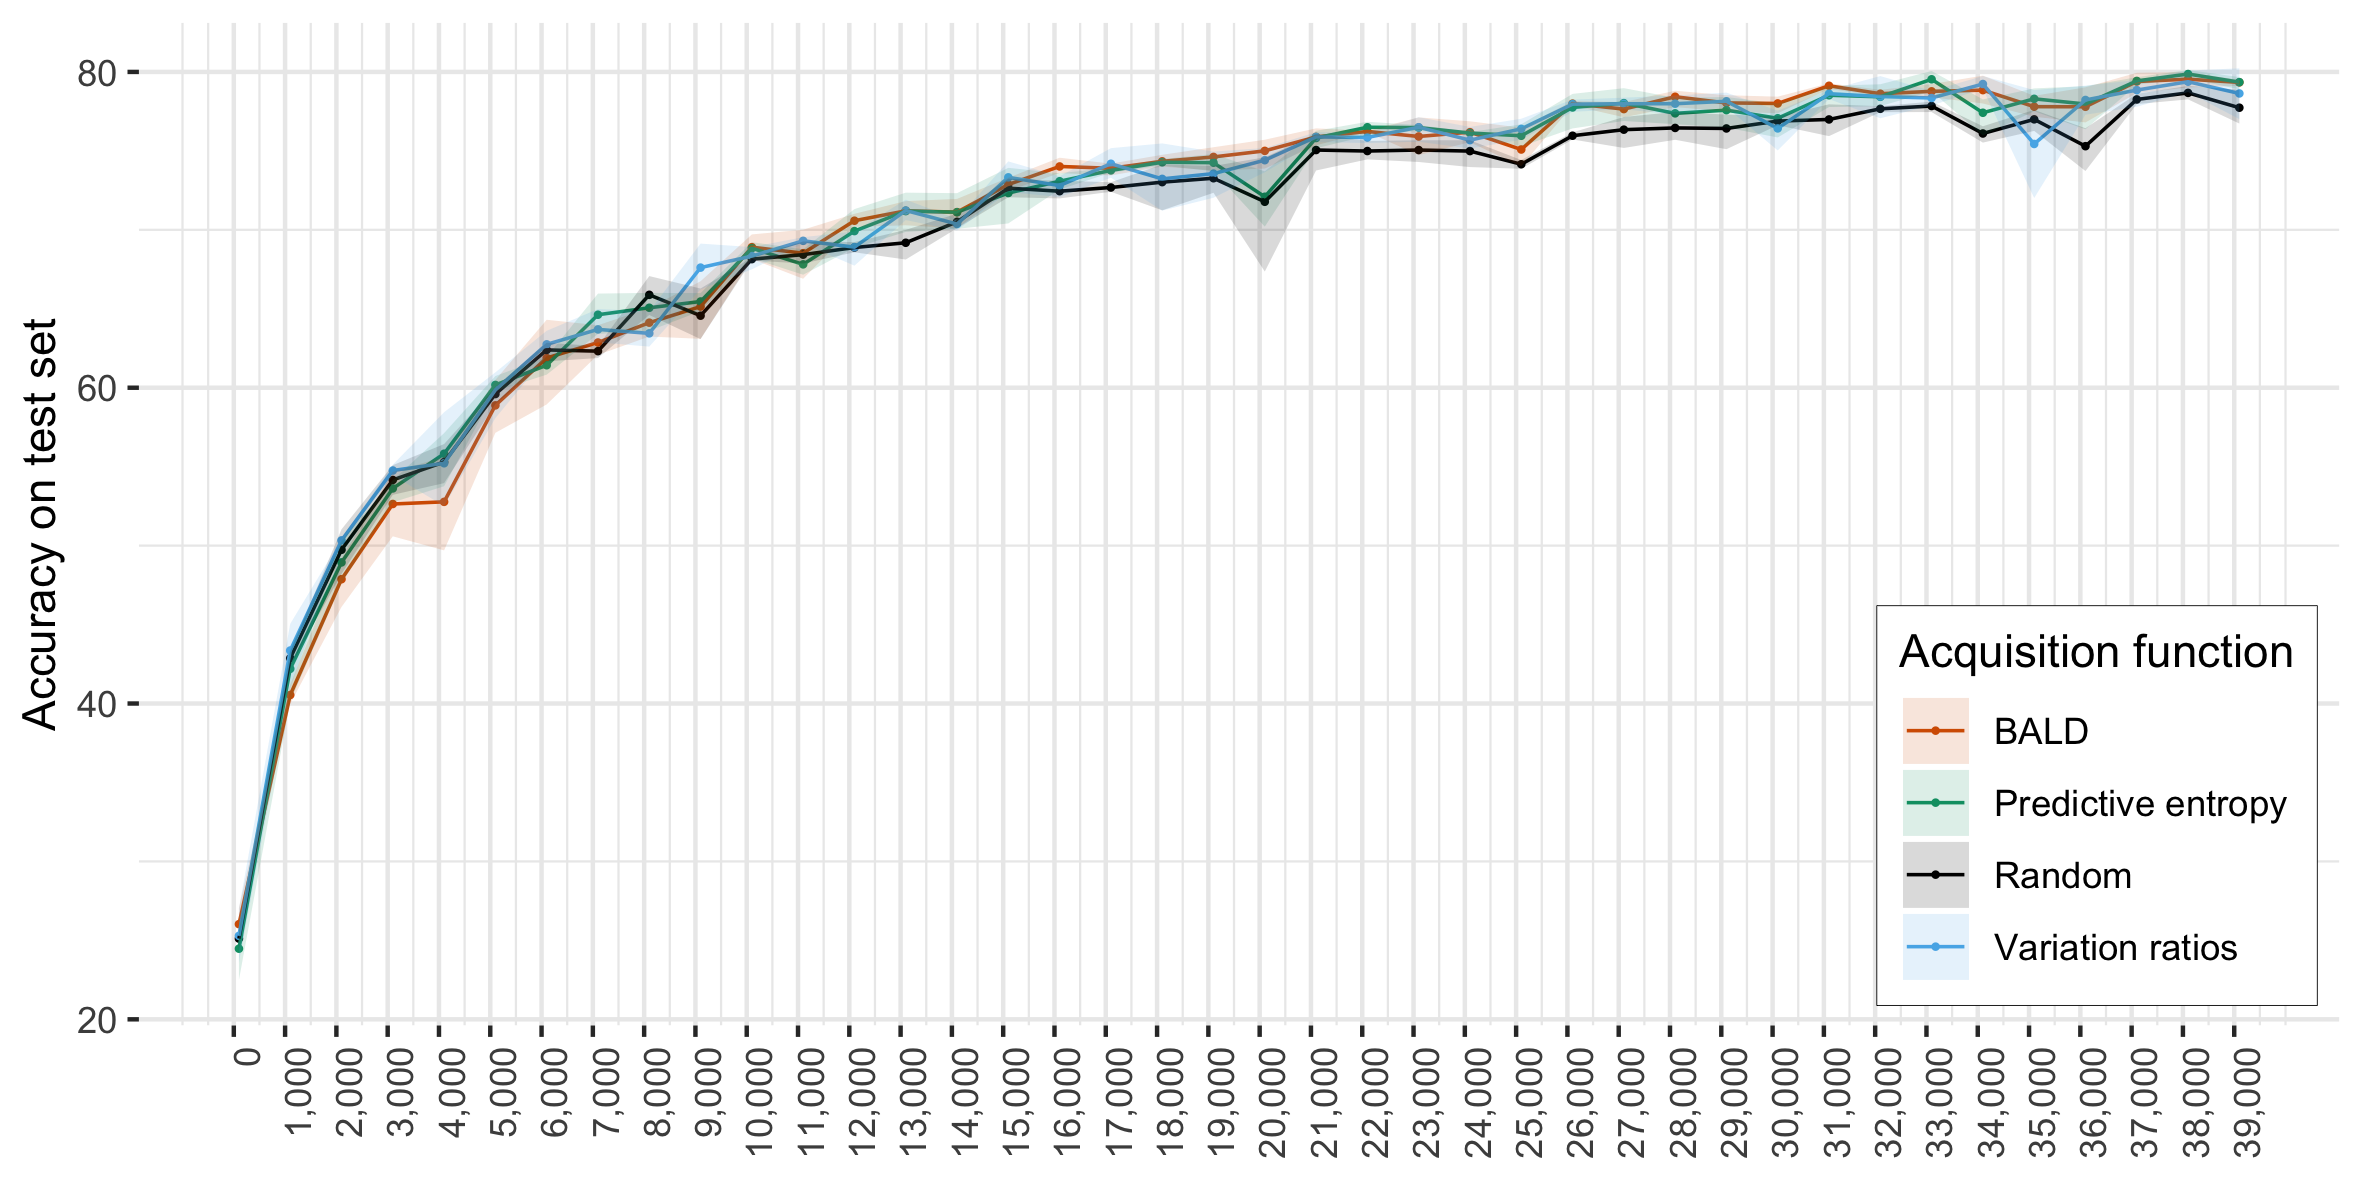
\includegraphics[width=\textwidth]{CIFAR10_accuracies_bayesian_shaded}
    \caption{Accuracy of models in each acquisition step in the CIFAR10 dataset.}
    \label{fig:CIFAR10_accuracies_bayesian}
\end{figure}

Figure \ref{fig:CIFAR10_bayesian_vs_freq} shows the comparison of the frequentist and Bayesian acquisition functions, with predictive entropy on the left and variation ratios on the right. As with the MNIST and with the cats and dogs datasets, the distinction between the frequentist and the Bayesian acquisition functions is not clear.

\begin{figure}[H]
    \centering
    \subfloat[Predictive entropy.]{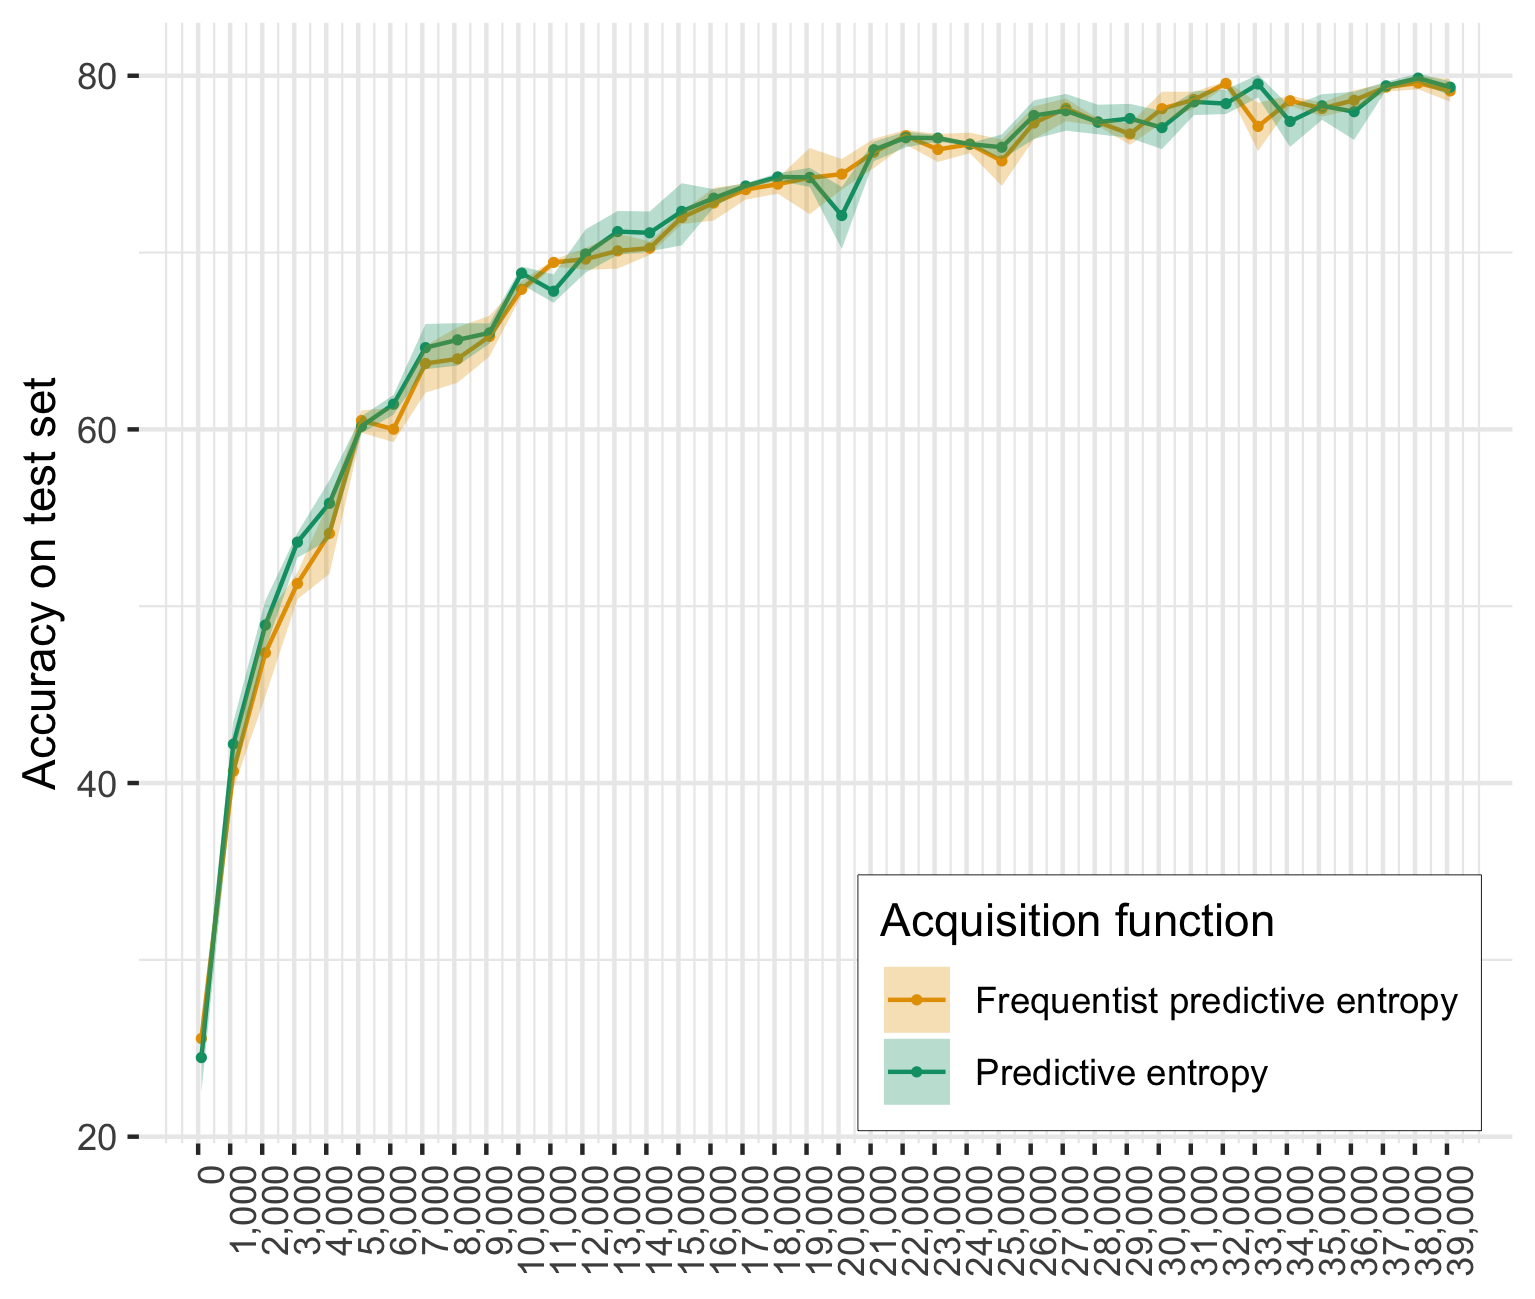
\includegraphics[width=0.5\textwidth]{CIFAR10_accuracies_pred_ent_ribbon}}
    \hfill
    \subfloat[Variation ratios.]{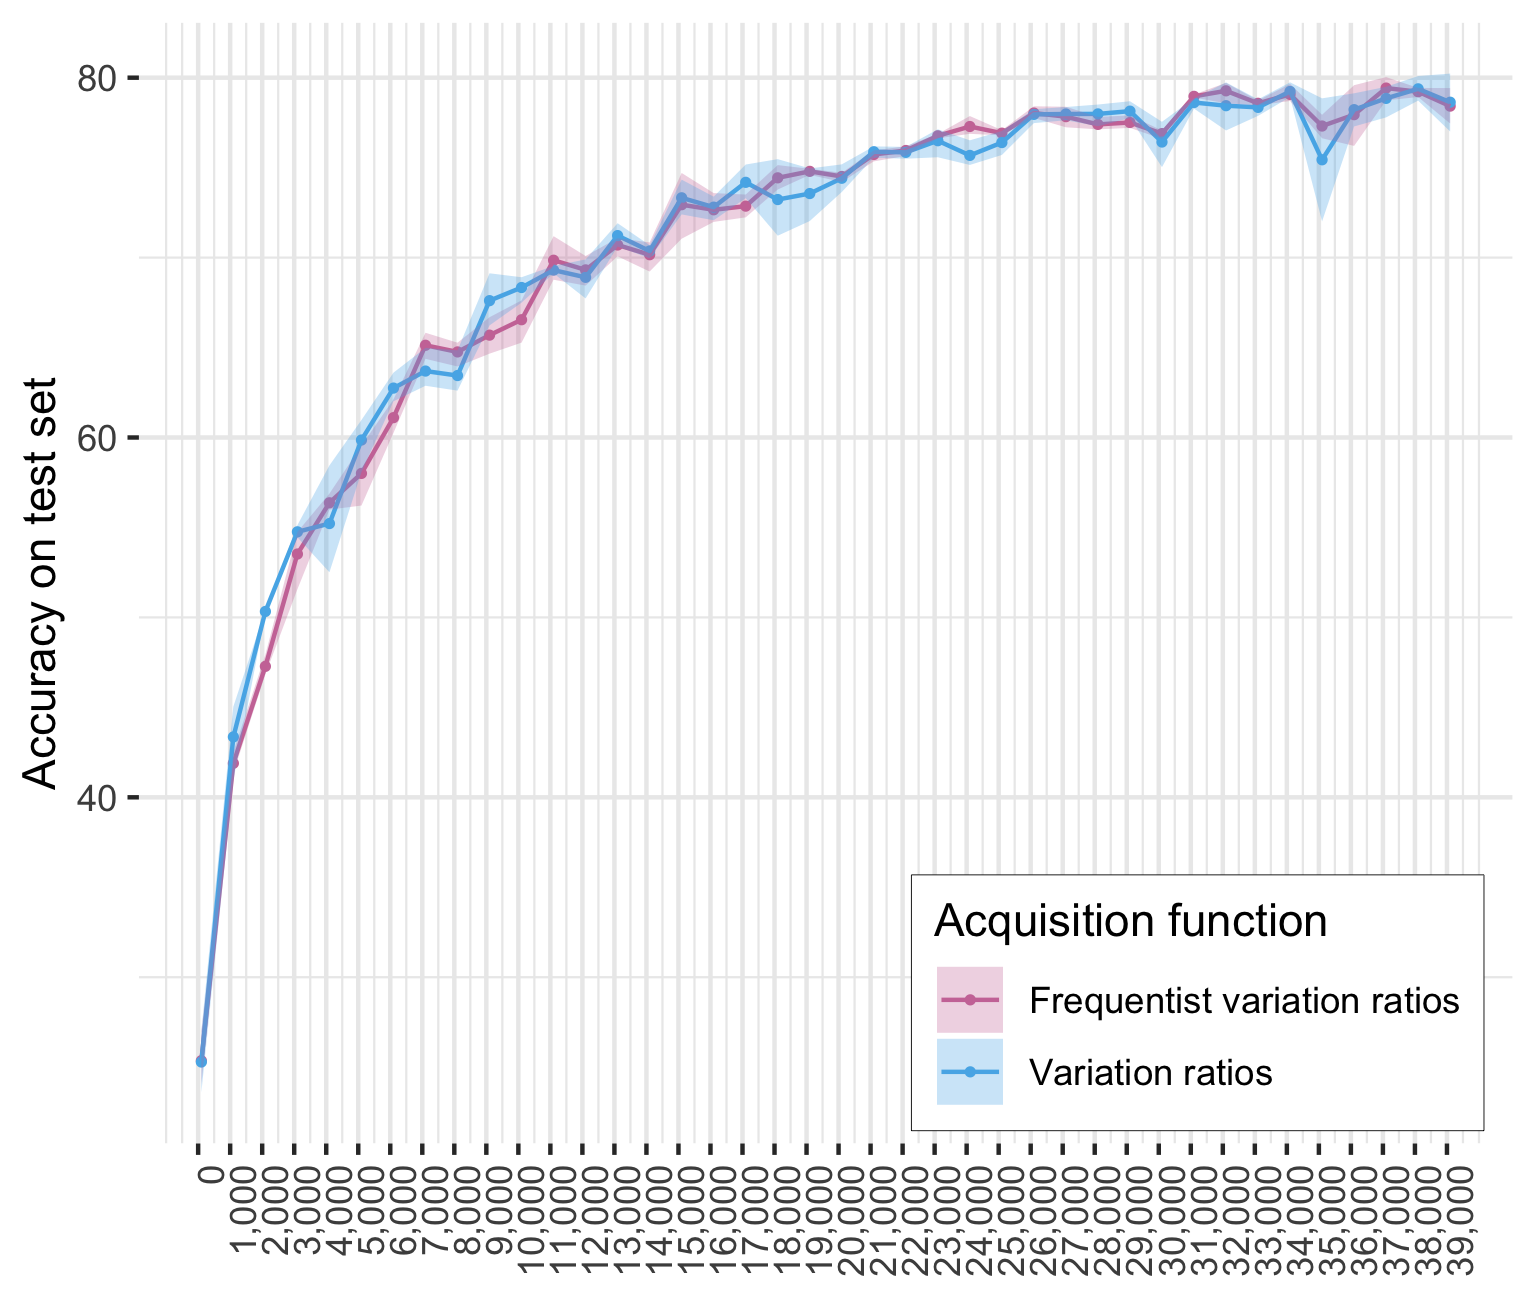
\includegraphics[width=0.5\textwidth]{CIFAR10_accuracies_var_ratios_ribbon}}
    \caption{Accuracy of models in each acquisition step in the CIFAR10 dataset.}
    \label{fig:CIFAR10_bayesian_vs_freq}
\end{figure}



%%%%%%%%%%%%%%%%%%%%%%%%%%%%%%%%%%%%%%%%%%%%%%%%%%%%%%%%%%%%%%
%%%%%%%%%%%%%%%%%%%%%%%%%%%%%%%%%%%%%%%%%%%%%%%%%%%%%%%%%%%%%%
\section{Discussion}
%%%%%%%%%%%%%%%%%%%%%%%%%%%%%%%%%%%%%%%%%%%%%%%%%%%%%%%%%%%%%%
%%%%%%%%%%%%%%%%%%%%%%%%%%%%%%%%%%%%%%%%%%%%%%%%%%%%%%%%%%%%%%

In this chapter, the results of several Active Learning experiments using different acquisition functions in three different datasets were shown. In the MNIST dataset there is a clear improvement in using the predicted probabilities of a trained model to select the images to add to a training set when compared to a random selection. In the CIFAR10 dataset there seems to be a small performance improvement when using the non-random acquisition functions. In the cats and dogs dataset there is an even smaller performance improvement, but it is not as clear as in the MNIST dataset.

However, it should be noted that in the case of the CIFAR10 and the cats and dogs datasets, the problem is much more high-dimensional than in the MNIST case. In higher dimensions there is more space between images, which makes the active learning procedure behave more similarly to a random acquisition function.

In all cases, there is no clear distinction between using an approximate Bayesian model against a frequentist one, as the accuracies did not seem to be different. This again may be because of the dimensionality of the problems that are being solved. In general, finding posterior distributions of high-dimensional spaces is difficult. In addition to this, the theoretical approximation of Dropout to a Bayesian CNN does not specify the quality of the approximation. Perhaps in the cases that were tested in this work, the variational approximation is not good and, therefore, the uncertainty given by the Bayesian acquisition functions is very similar to that of the frequentist ones.

In the following chapter, final concluding remarks are discussed.
